\documentclass[a4paper,12pt,twoside]{memoir}

% Castellano
\usepackage[spanish,es-tabla]{babel}
\selectlanguage{spanish}
\usepackage[utf8]{inputenc}
\usepackage[T1]{fontenc}
\usepackage{lmodern} % Scalable font
\usepackage{microtype}
\usepackage{placeins}
\usepackage{eurosym}
\usepackage{cite}

\RequirePackage{booktabs}
\RequirePackage[table]{xcolor}
\RequirePackage{xtab}
\RequirePackage{multirow}

% Links
\usepackage[colorlinks]{hyperref}
\hypersetup{
	allcolors = {red}
}

% Ecuaciones
\usepackage{amsmath}

% Rutas de fichero / paquete
\newcommand{\ruta}[1]{{\sffamily #1}}

% Párrafos
\nonzeroparskip


% Imagenes

\usepackage{graphicx}
\usepackage{wrapfig}
\newcommand{\imagen}[2]{
	\begin{figure}[!h]
		\centering
		\includegraphics[width=0.9\textwidth]{#1}
		\caption{#2}\label{fig:#1}
	\end{figure}
	\FloatBarrier
}

\newcommand{\imagenflotante}[2]{
	\begin{figure}%[!h]
		\centering
		\includegraphics[width=0.9\textwidth]{#1}
		\caption{#2}\label{fig:#1}
	\end{figure}
}



% El comando \figura nos permite insertar figuras comodamente, y utilizando
% siempre el mismo formato. Los parametros son:
% 1 -> Porcentaje del ancho de página que ocupará la figura (de 0 a 1)
% 2 --> Fichero de la imagen
% 3 --> Texto a pie de imagen
% 4 --> Etiqueta (label) para referencias
% 5 --> Opciones que queramos pasarle al \includegraphics
% 6 --> Opciones de posicionamiento a pasarle a \begin{figure}
\newcommand{\figuraConPosicion}[6]{%
  \setlength{\anchoFloat}{#1\textwidth}%
  \addtolength{\anchoFloat}{-4\fboxsep}%
  \setlength{\anchoFigura}{\anchoFloat}%
  \begin{figure}[#6]
    \begin{center}%
      \Ovalbox{%
        \begin{minipage}{\anchoFloat}%
          \begin{center}%
            \includegraphics[width=\anchoFigura,#5]{#2}%
            \caption{#3}%
            \label{#4}%
          \end{center}%
        \end{minipage}
      }%
    \end{center}%
  \end{figure}%
}

%
% Comando para incluir imágenes en formato apaisado (sin marco).
\newcommand{\figuraApaisadaSinMarco}[5]{%
  \begin{figure}%
    \begin{center}%
    \includegraphics[angle=90,height=#1\textheight,#5]{#2}%
    \caption{#3}%
    \label{#4}%
    \end{center}%
  \end{figure}%
}
% Para las tablas
\newcommand{\otoprule}{\midrule [\heavyrulewidth]}
%
% Nuevo comando para tablas pequeñas (menos de una página).
\newcommand{\tablaSmall}[5]{%
 \begin{table}
  \begin{center}
   \rowcolors {2}{gray!35}{}
   \begin{tabular}{#2}
    \toprule
    #4
    \otoprule
    #5
    \bottomrule
   \end{tabular}
   \caption{#1}
   \label{tabla:#3}
  \end{center}
 \end{table}
}

%
% Nuevo comando para tablas pequeñas (menos de una página).
\newcommand{\tablaSmallSinColores}[5]{%
 \begin{table}[H]
  \begin{center}
   \begin{tabular}{#2}
    \toprule
    #4
    \otoprule
    #5
    \bottomrule
   \end{tabular}
   \caption{#1}
   \label{tabla:#3}
  \end{center}
 \end{table}
}

\newcommand{\tablaApaisadaSmall}[5]{%
\begin{landscape}
  \begin{table}
   \begin{center}
    \rowcolors {2}{gray!35}{}
    \begin{tabular}{#2}
     \toprule
     #4
     \otoprule
     #5
     \bottomrule
    \end{tabular}
    \caption{#1}
    \label{tabla:#3}
   \end{center}
  \end{table}
\end{landscape}
}

%
% Nuevo comando para tablas grandes con cabecera y filas alternas coloreadas en gris.
\newcommand{\tabla}[6]{%
  \begin{center}
    \tablefirsthead{
      \toprule
      #5
      \otoprule
    }
    \tablehead{
      \multicolumn{#3}{l}{\small\sl continúa desde la página anterior}\\
      \toprule
      #5
      \otoprule
    }
    \tabletail{
      \hline
      \multicolumn{#3}{r}{\small\sl continúa en la página siguiente}\\
    }
    \tablelasttail{
      \hline
    }
    \bottomcaption{#1}
    \rowcolors {2}{gray!35}{}
    \begin{xtabular}{#2}
      #6
      \bottomrule
    \end{xtabular}
    \label{tabla:#4}
  \end{center}
}

%
% Nuevo comando para tablas grandes con cabecera.
\newcommand{\tablaSinColores}[6]{%
  \begin{center}
    \tablefirsthead{
      \toprule
      #5
      \otoprule
    }
    \tablehead{
      \multicolumn{#3}{l}{\small\sl continúa desde la página anterior}\\
      \toprule
      #5
      \otoprule
    }
    \tabletail{
      \hline
      \multicolumn{#3}{r}{\small\sl continúa en la página siguiente}\\
    }
    \tablelasttail{
      \hline
    }
    \bottomcaption{#1}
    \begin{xtabular}{#2}
      #6
      \bottomrule
    \end{xtabular}
    \label{tabla:#4}
  \end{center}
}

%
% Nuevo comando para tablas grandes sin cabecera.
\newcommand{\tablaSinCabecera}[5]{%
  \begin{center}
    \tablefirsthead{
      \toprule
    }
    \tablehead{
      \multicolumn{#3}{l}{\small\sl continúa desde la página anterior}\\
      \hline
    }
    \tabletail{
      \hline
      \multicolumn{#3}{r}{\small\sl continúa en la página siguiente}\\
    }
    \tablelasttail{
      \hline
    }L
    \bottomcaption{#1}
  \begin{xtabular}{#2}
    #5
   \bottomrule
  \end{xtabular}
  \label{tabla:#4}
  \end{center}
}

\definecolor{cgoLight}{HTML}{EEEEEE}
\definecolor{cgoExtralight}{HTML}{FFFFFF}

%
% Nuevo comando para tablas grandes sin cabecera.
\newcommand{\tablaSinCabeceraConBandas}[5]{%
  \begin{center}
    \tablefirsthead{
      \toprule
    }
    \tablehead{
      \multicolumn{#3}{l}{\small\sl continúa desde la página anterior}\\
      \hline
    }
    \tabletail{
      \hline
      \multicolumn{#3}{r}{\small\sl continúa en la página siguiente}\\
    }
    \tablelasttail{
      \hline
    }
    \bottomcaption{#1}
    \rowcolors[]{1}{cgoExtralight}{cgoLight}

  \begin{xtabular}{#2}
    #5
   \bottomrule
  \end{xtabular}
  \label{tabla:#4}
  \end{center}
}

\graphicspath{ {./img/} }

% Capítulos
\chapterstyle{bianchi}
\newcommand{\capitulo}[2]{
	\setcounter{chapter}{#1}
	\setcounter{section}{0}
	\chapter*{#2}
	\addcontentsline{toc}{chapter}{#2}
	\markboth{#2}{#2}
}

% Apéndices
\renewcommand{\appendixname}{Apéndice}
\renewcommand*\cftappendixname{\appendixname}

\newcommand{\apendice}[1]{
	%\renewcommand{\thechapter}{A}
	\chapter{#1}
}

\renewcommand*\cftappendixname{\appendixname\ }

% Formato de portada
\makeatletter
\usepackage{xcolor}
\newcommand{\tutor}[1]{\def\@tutor{#1}}
\newcommand{\course}[1]{\def\@course{#1}}
\definecolor{cpardoBox}{HTML}{E6E6FF}
\def\maketitle{
  \null
  \thispagestyle{empty}
  % Cabecera ----------------
\noindent
\includegraphics[width=\textwidth]{cabecera}\vspace{1cm}%
  \vfill
  % Título proyecto y escudo informática ----------------
  \colorbox{cpardoBox}{%
    \begin{minipage}{.8\textwidth}
      \vspace{.5cm}\Large
      \begin{center}
      \textbf{TFG del Grado en Ingeniería Informática}\vspace{.6cm}\\
      \textbf{\LARGE\@title{}}
      \end{center}
      \vspace{.2cm}
    \end{minipage}

  }%
  \hfill\begin{minipage}{.20\textwidth}
    
\includegraphics[width=\textwidth]{escudoInfor}
  \end{minipage}
  \vfill
  % Datos de alumno, curso y tutores ------------------
  \begin{center}%
  {%
    \noindent\LARGE
    Presentado por \@author{}\\ 
    en la Universidad de Burgos --- \@date{}\\
    \@tutor{}\\
  }%
  \end{center}%
  \null
  \cleardoublepage
  }
\makeatother

\newcommand{\nombre}{Eduardo Rodríguez Soto} %%% cambio de comando
\newcommand{\nombreTutor}{Tutor académico: Ángel Arroyo Puente\\
Tutor empresarial en HP: Pablo Tejedor García}

% Datos de portada
\title{ Aplicación de tecnología Blockchain a una cadena de distribución de productos}
\author{\nombre}
\tutor{\nombreTutor}
\date{\today}

\begin{document}

\maketitle

%%%%%%%%%%%%%%%%%%%%%%%%%%%%%%%%%%%%%%%%%%%%%%%%%%%%%%%%%%%%%%%%%%%%%%%%%%%%%%%%%%%%%%%%


\noindent
\includegraphics[width=\textwidth]{cabecera}\vspace{1cm}

\noindent D. Ángel Arroyo Puente, profesor del departamento de Ingeniería Civil, área de Lenguajes y Sistemas Informáticos.

\noindent Expone:

\noindent Que el alumno D. \nombre, con DNI: 71293020-N, ha realizado el Trabajo final de Grado en Ingeniería Informática titulado: Aplicación de tecnología Blockchain a una cadena de distribución de productos. 

\noindent Y que dicho trabajo ha sido realizado por el alumno bajo la dirección del que suscribe, en virtud de lo cual se autoriza su presentación y defensa.

\begin{center} %\large
En Burgos, {\large \today}
\end{center}

\vfill\vfill\vfill

% Author and supervisor
\begin{minipage}{0.45\textwidth}
\begin{flushleft} %\large
Vº. Bº. del Tutor académico:\\[2cm]
D. Ángel Arroyo Puente
\end{flushleft}
\end{minipage}
\hfill
\begin{minipage}{0.45\textwidth}
\begin{flushleft} %\large
Vº. Bº. del tutor empresarial :\\[2cm]
D. Pablo Tejedor García
\end{flushleft}
\end{minipage}
\hfill

\vfill


\frontmatter

% Abstract en castellano
\renewcommand*\abstractname{Resumen}
\begin{abstract}

Este trabajo ha sido realizado con la Universidad de Burgos y la empresa \textit{Hewlett-Packard HP}, en su sede ubicada en León. 

La compañía HP se dedica a la fabricación y comercialización de \textit{hardware} y \textit{software}. Otro servicio destacable que ofrece HP es la asistencia a sus usuarios.

La empresa HP con sede en León tiene como objetivo el desarrollo de software para impresoras de largo formato. Los productos que se investigan y desarrollan  en el centro están relacionados con el firmware de las máquinas así como con los programas que permiten el uso de las mismas a aplicaciones y sistemas operativos.

El rango de productos de largo formato va desde impresoras A3 a impresoras 3D pasando por máquinas de producción industrial y máquinas gráficas o diseño (usadas principalmente en estudios de arquitectura e ingeniería).

El principal propósito de este trabajo es el desarrollo de una página web con el fin de que un usuario concreto pueda interactuar con la tecnología blockchain y, así, poder llevar a cabo las diferentes opciones que nos ofrece la página web, como son:

\begin{itemize}
	\item Crear de usuarios.
	\item Añadir un producto.
	\item Consultar todos los productos que tiene dicho cliente.
\end{itemize}

Este trabajo se ha realizado con la herramienta de trabajo VisualStudio Code, para la implementación de la página web, y con la herramienta Metamask , para la creación de los contratos.

\end{abstract}

\renewcommand*\abstractname{Descriptores}
\begin{abstract}
Html, Php, tecnología blockchain, Metamask, Ganache, Remix
\end{abstract}

\clearpage

% Abstract en inglés
\renewcommand*\abstractname{Abstract}
\begin{abstract}
This work has been carried out with the University of Burgos and the Hewlett-Packard HP company located in the city of León.  

HP is engaged in the manufacture and commercialization of hardware and software. Another noteworthy service offered by HP is the assistance to its users.

HP León is dedicated to at developing software for long-format printers. The products that are researched and developed in the center are related to the firmware of the machines as well as to the programs that allow the use of them to applications and operating systems. 
 
The range of long format products ranges from A3 printers to 3D printers to industrial production machines and graphics or design machines (mainly used in architectural and engineering studies). 
 
The main purpose of this work is the development of a web page in order for a specific user to interact with blockchain technology and, thus, be able to carry out the different options offered by the web address, such as: 

\begin{itemize}
	\item Create users.
	\item Add a product. 
	\item Consult all the products that the customer has. 
\end{itemize}

This work has been done with the VisualStudio Code working tool, for the implementation of the web page, and with the Metamask tool, for the creation of contracts.

\end{abstract}

\renewcommand*\abstractname{Keywords}
\begin{abstract}
Html, Php, tecnología blockchain, Metamask, Ganache, Remix
\end{abstract}

\clearpage

% Indices
\tableofcontents

\clearpage

\listoffigures

\clearpage

%\listoftables


\mainmatter
\capitulo{1}{Introducción}

La empresa HP con sede en León tiene como objetivo el desarrollo de software para impresoras de largo formato. Los productos que se investigan y desarrollan en este centro están relacionados con el \textit{firmware} de las máquinas así como con los programas que permiten el uso de las mismas a aplicaciones y sistemas operativos.

En los últimos tiempos, HP ha creado una nueva unidad de trabajo a la cual se la denomina grupo de innovación y consiste en explorar nuevas tecnologías. Una de las tecnologías a investigar es la tecnología Blockchain, de la que explicaremos en este documento. 

Blockchain\cite{informacionB} surge en 1991 de la mano de \textit{Stuart Haber} y \textit{W. Scott Stornetta}, ambos científicos crearon la tecnología de las criptomonedas más conocida como cadena de bloques (esto permite a cada cliente de la red poder hacer una transferencia a otra persona sin tener que confiar entre sí). Para dar más seguridad, un año después se incorporan los árboles Merkle\footnote{Árbol de \textit{Merkle}: es una estructura de árbol, en el que cada nodo que no es una hoja le corresponde una etiqueta hash de la concatenación de las etiquetas de los nodos hijo.}, lo que hace esta tecnología es que sea más eficaz y rugoso ya que permite que varios archivos o documentos se puedan juntar todos en un mismo bloque. En el año 2004, se introducen los sistemas RPoW (Prueba de trabajo Reutlizable), que resuelve el problema de doble gasto, en el 2008 se crea la red Bitcoin y en 2013 nace la red Ethereum.

Uno de los objetivos del presente proyecto es la creación de una página web, esta página la realizaremos en un servidor local llamado XAMPP, primeramente tendremos que instalar XAMPP (se explicará en el apartado de los anexos) esto será nuestra base de datos, con la cual guardaremos a los usuarios que se registren desde la página, desde la página tendremos opción de modificar y borrar los usuarios. 

Cuando el usuario se haya registrado, tendremos la posibilidad de realizar los smart contract, es un contrato que es capaz de ejecutarse y hacerse cumplir por sí mismo, de manera autónoma y automática, sin intermediarios ni mediadores, que conectará a un sistema de red privada llamada Rospten, y le pasaremos diferentes parámetros, una vez creado no se podrán ni modificar ni destruir. 

La realización de todas las pruebas ha ido cambiando desde la creación de diferentes \textit{smart contract} tanto en la red local (Ganache), en cuentas privadas (Ropsten) e incluso en la red principal de Ethereum. La realización de los \textit{smart contract} es mediante metamask, web3, node.js, solidity y más aplicaciones que explicaremos más detalladamente en los siguientes puntos.

\subsection{Estructura de la memoria}

Esta memoria constará de los contenidos explicados a continuación:

\begin{enumerate}[1)]
\item \textbf{Resumen}: breve introducción de los objetivos y descripción de la empresa con la cual realizo dicho trabajo. Este apartado estará tanto en castellano como en inglés. 
\item \textbf{Objetivos del proyecto}: se detallarán los objetivos qeu se quieren conseguir al realizar este proyecto.
\item \textbf{Conceptos teóricos}: realizamos un pequeño resumen de los conceptos que hemos aprendido al realizar dicho proyecto.
\item \textbf{Técnicas y herramientas}: descripción de los programas utilizados para la elaboración y seguimiento del proyecto.
\item \textbf{Aspectos relevantes del desarrollo del proyecto}: aclaración de las herramientas utilizadas y argumentación final de nuestro proyecto.
\item \textbf{Trabajos relacionados}: consiste en hablar de los trabajos similares a nuestro trabajo, tanto realizados por la universidad de Burgos o ajenos a ella.
\item \textbf{Conclusiones y líneas de trabajo futuras}: valoración de todo lo conseguido y posibles mejoras que se podrán mejorar en futuros trabajos relacionados con este proyecto.
\item \textbf{Bibliografía}: información encontrada en Internet, a la que se hace referencia en cada apartado usado en la memoria del proyecto. 
\end{enumerate}

\subsection{Estructura de los anexos}

Los anexos se estructuran de la siguiente manera:

\begin{enumerate}[1)]
	\item \textbf{Plan de proyecto de software}: estudio de la viabilidad tanto legal como económica del proyecto, también comentaremos los objetivos propuestos en cada reunión.
	\item \textbf{Especificación de usuarios}: en este apartado explicaremos los
casos de uso y requisitos funcionales de la herramienta creada.
	\item \textbf{Especificación de diseño}: se detallaran los diseños software utilizados en este proyecto.
	\item \textbf{Documentación técnica de programación}: explicación de la instalación del programa y guia del código fuente mas relevante.
	\item \textbf{Manual de usuario}: guía para el manejo de la aplicación para cualquier usuario, requisitos e instalación.
\end{enumerate}

\subsection{Contenido entregable en el CD}

Los documentos que contiene el CD serán:

\begin{enumerate}
\item Documentación de la memoria: versión en \textit{pdf} de la memoria final.
\item Documentación de los anexos: versión en \textit{pdf} de la anexos finales.
\item Código del programa: version final del código ejecutable para la puesta en marcha del trabajo.
\item Vídeo explicativo de las funcionalidades de la página web.
\end{enumerate}


\capitulo{2}{Objetivos del proyecto}

El objetivo de este trabajo es la creación de una página web y la investigación es indagar sobre las posibilidades de la tecnología blockchain y su posible aplicación en las unidades de negocio de HP.

Los trabajos de observatorio son gestionados por una nueva unidad de trabajo de HP León denominada ``grupo de innovación'' cuya misión es explorar nuevas tecnologías que permitan mejorar los procesos de desarrollo o ampliar los campos de negocio de la compañía.

\section{Objetivos Técnicos y Generales}

\begin{enumerate}[1]
	\item Explorar las posibilidades de la tecnología blockchain.
	\item Explorar las posibilidades y capacidades de la red \textit{ethereum} y \textit{solidity} para desarrollar smart contracts.
	\item Ampliar conocimientos del alumno en la tecnología blockchain.
	\item Creación de la página web, con el fin de conseguir la conexión entre la plataforma Ethereum y nuestra página mediante el uso de Metamask.
	\item Familiarizar al alumno con las metodologías ágiles como \textit{SCRUM}.
	\item Permitir al alumno conocer los métodos de trabajo de la compañía HP.
	\item Familiarizar al alumno con las metodologías ágiles como \textit{SCRUM}.
\end{enumerate}
\capitulo{3}{Conceptos teóricos \textit{Scrum}}

Después de analizar diferentes fuentes bibliográfica, se ha decidido tomar como referencia el libro \textit{[Scrum y xp desde las trincheras]}``[Henrik Kniberg, 2018]''\cite{libro} como principal fuente de información.

\section{Introducción}

\textit{Scrum} es una herramienta ágil de trabajo creada por Ken Schwaber, quien defendió que Scrum no era una metodología de trabajo, sino que más bien era un marco de trabajo. Es decir, este sistema explicaba los pasos que se deben seguir para realizar un trabajo con éxito. El autor esclareció que Scrum era un vía a la que adaptarse según la situación concreta en la que se fuera a trabajar, puesto que cada proyecto puede contar con particularidades. De todas formas, el objetivo del libro es desarrollar una forma de trabajo más eficiente y productiva.

En los siguientes apartados pretendemos, analizar el libro, todo ellos desde la visión de la persona que escribió el libro, el sueco Henrik Kniberg.

\section{Cómo hacemos las pilas de producto}

La lista de producto es la parte más importante del \textit{Scrum}. Aquí comienza a funcionar todo el proyecto, en esta lista se incluyen los principales objetivos de los requisitos que se quieren conseguir al final del proyecto, a esto lo llama elementos de la pila o historias.

Elementos de la pila:
\begin{itemize}
	\item \underline{ID}: es el identificador único, contador de los elementos o historias.
	\item \underline{Nombre}: breve explicación del problema a tratar será clara y concisa.
	\item \underline{Importancia}: ratio de consideración que el dueño dé a cada
	elemento.
	\item \underline{Estimación inicial}: valoración del equipo de cuánto trabajo es
	necesario para cada tarea.
	\item \underline{Como probarlo}: realización de pruebas o \textit{demos} en el  \textit{sprint} final, ej.
	realización de pruebas o test.
	\item \underline{Notas}: información que pueda considerarse aclaratoria, o que haga
\end{itemize}

Estos seis campos mencionados son aquellos que más importancia se les da a la hora de realizar los \textit{sprint}. Para la realización de estos campos en los diferentes trabajos académicos es importante realizar los trabajos en tablas Excel, las cuales podrían ver simultáneamente tanto el dueño como los múltiples usuarios.


De la misma manera, el autor menciona que se pueden usar unos elementos adicionales que pueden mejorar la accesibilidad por parte del dueño y así controlarlo mejor las propiedades de cada apartado. Estos campos son: \textbf{la categoría} explicación de la historia básica, \textbf{componentes} realización de tickets para comprobar si los procesos se cumplen, \textbf{solicitante} indicar los avances del producto y \textbf{bug tracking id} seguimiento de errores reportados.

\section{Cómo nos preparamos y planificamos un \textit{sprint}}
Llegados a este punto las preparaciones de los \textit{sprint} se aproximan y lo más importante es tener la pila del producto correctamente lista antes de la planificación del  \textit{sprint}.
Esto quiere decir que es necesario intentar conseguir unos objetivos antes de empezar la
planificación:
\begin{itemize}
	\item Deberá existir la pila del producto.
	\item Habrá una pila de producto y un dueño de producto.
	\item Tendrá los ratios de importancia bien definidos (independientemente de que puedan
coincidir algunos de los ratios para las tareas menos importantes).
 	\item El dueño del producto es el que dará importancia de cada cosa.
\end{itemize}

Una vez concluida la preparación, es momento de desarrollar la planificación, que consiste en realizar una reunión, la que se convertirá en la más decisiva del \textit{scrum}. Si la reunión fuera mal ejecutada podría arruinar por completo el \textit{sprint}, el objetivo de esta planificación de \textit{sprint} es dar al equipo la información necesaria para poder trabajar durante las siguientes semanas.

Los objetivos de la planificación del \textit{sprint} son: establecer la meta, elegir a los miembros con la dedicación que tendrán y realizar la pila del \textit{sprint} (incluyendo las historias). También es adecuado elegir el lugar y la fecha para la reuniones de las celebraciones de los \textit{sprint} diario.

El dueño del producto, por regla, no suele asistir a las reuniones y no trabaja con el equipo, aunque, es recomendable que asista ya que pueden darse tres variables interdependientes, como muestra la figura \ref{triangulo}.

\begin{wrapfigure}{r}{0.4\linewidth}
    \centering
    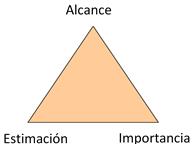
\includegraphics[width=0.30\textwidth]{triagulovariables}
    \caption{Triangulo de variables}
    \label{triangulo}
\end{wrapfigure}

El alcance y la importancia son fijados por el dueño de producto. La estimación la proporciona el equipo de trabajo.

Cuando se planifica el \textit{sprint}, estas variables sufren un desajuste continuo con cada dialogo que se produce cara a cara entre el equipo y el dueño del producto.

En el triángulo antes expuesto faltaría un último elemento que sería la calidad. Esta se subdivide en dos categorías: calidad externa e interna, la primera la perciben los usuarios del sistema y se trata de una interfaz lenta y poco intuitiva, por otro lado, dentro de la calidad interna se encuentran los aspectos no visible al usuario, pero con gran efecto en la mantenibilidad del sistema, como consistencia, refactorización. La segunda es algo alcanzable y la calidad interna es algo que no puede ser discutido.

En las reuniones, el dueño de producto explica cuáles son los objetivos del \textit{sprint} y las historias más importantes a conseguir. El equipo las repasa y las asigna un tiempo estimado de ejecución.

Si el dueño no se presentara a las reuniones, se propondría a alguien del grupo para que desempeñara las funciones de delegado durante las reuniones. Si no surgiera un sustituto, se intentaría asignar un nuevo dueño del proyecto y, por último, se pospondrían los lanzamientos del \textit{sprint} hasta que el dueño esté disponible y pueda asistir a las reuniones.

\subsection{\textbf{Reuniones de planificación de \textit{Sprint} que duran}}

Los \textit{scrum} tienen una duración determinada (\textit{time-boxed}). Cuando una reunión de planificación de \textit{sprint} está llegando al final y aún no están todos los objetivos cumplidos, ¿qué se aconseja hacer? se recomienda la opción de dar la reunión por finalizada. La reunión perdería parte de su utilidad y con esto conseguimos que en la siguiente reunión los \textit{sprint} sean más eficientes y se ofrezca menos resistencia cuando se proponga una duración excesiva.

Se recomienda que las reuniones sean lo más ágiles posible, aunque los sprint largos pueden resultar beneficiosos ya que prestan más tiempo a la detección de errores. Aproximadamente tienen una duración de tres semanas.

\subsection{\textbf{¿Qué historias incluir en un \textit{Sprint}?}}

Al principio de las reuniones se intentan poner unos objetivos en común (historias) con la importancia de cada una de ellas; estas se pondrán en orden de mayor a menor. El grupo de trabajo intentará agrupar el número de historias convenientes según ellos estimen que serán
capaces de realizar en la duración de un\textit{sprint}.

Tendremos la lista de las tareas por realizar en la pila del producto y serán incluidas en la pila del \textit{Sprint}, como se puede ver en la siguiente fotografía.

\begin{wrapfigure}{l}{0.3\linewidth}
    \centering
    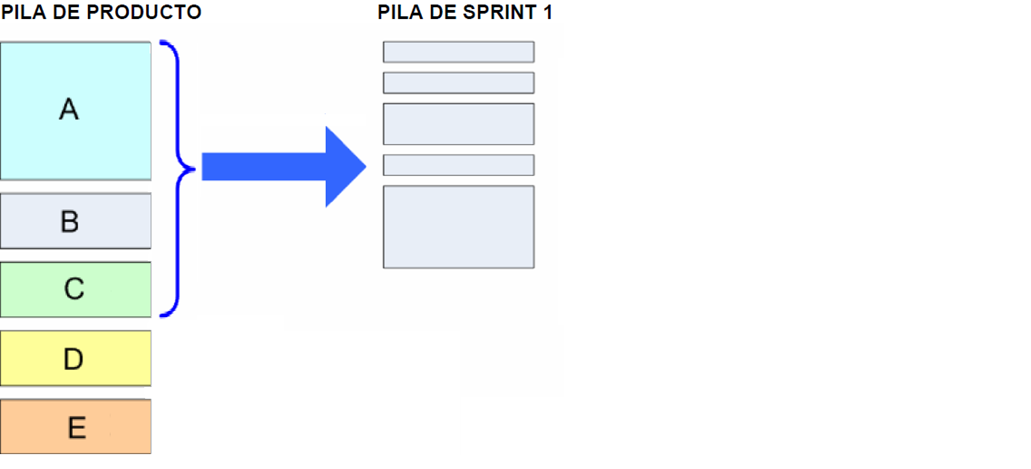
\includegraphics[width=0.45\textwidth]{pasosSprint}
    \caption{Pasos de un \textit{sprint}}
\end{wrapfigure}

En el supuesto de que se quieren meter las tareas A, B y C, pero el dueño del producto quiera introducir la tarea D, una de las posibles combinaciones a realizar es: reorganizar la lista y dejar alguna de las tareas que tenemos fuera. Por ejemplo, nos quedaría A, B y D y se dejaría la tarea C fuera de la pila.

También se podría realizar el reparto de otras formas.\\


El equipo decide qué historias incluir mediante dos cálculos:
\begin{enumerate}
	\item Como se dice tradicionalmente,``a ojo de buen cubero'': suele darse para equipos pequeños y con \textit{sprint} cortos, se calculan suponiendo la dificultad de cada uno de ellos.
	\item Cálculos de velocidad:
	 \begin{enumerate}[a)]
	 	\item \underline{Decir la velocidad estimada}: medida de cantidad de trabajo realizado donde se evalúa en función de la estimación inicial
	 	\item \underline{Calculando las historias que se pueden añadir sin sobrepasar las velocidades}: la velocidad es una medida de cantidad de trabajo realizado, en la cual cada elemento se valora por la estimación que se hizo inicialmente.
	 	Una forma de realizar los cálculos de los recursos será mediante fórmulas, las cuáles son:
	 	\begin{description}
	 		\item [Días – hombre disponible]: Sumaremos los días que emplearan todos los trabajadores del proyecto (días/hombres disponibles).
	 		\begin{enumerate}
	 			\item \underline{Velocidad estimada}:  es igual a la disponibilidad de hombres y días junto al factor de dedicación, que depende de la concentración del equipo. Para calcular un buen factor estudiaremos cómo fueron los anteriores sprint.
	 			\item \underline{Factor de dedicación del ultimo \textit{sprint}}: es igual a la velocidad real repartida entre los días y hombres disponibles.
	 		\end{enumerate}
 		\end{description}
 	\item \underline{Uso de tarjetas}: con este método se logra que todos los integrantes del grupo sean participes y así dar el tiempo de realización de cada actividad.
 	\item Una vez que el equipo tiene definidas todas las tareas, estas se pasarán a una hoja de cálculo  para ver el avance de todo ello.
    \end{enumerate}
	\item Definición de terminado
	
	El primer caso que debe darse para que se considere como acabado es 	que el equipo este de acuerdo con esta decisión. Una historia se considera terminada cuando el encargado del \textit{scrum} así lo determina.
	 
	\item Estimación de tiempos con \textit{PLANNING POKER}
	
	En este tipo de estimación todos los miembros del equipo deben involucrarse para estimar cada historia ya que no sabemos quién implementará cada historia o si esa tarea la realizaran personas de diferentes áreas.
	
	Para ello existe el \textit{planning Poker}, diseñado por Mike Cohn. Esto consiste en cada miembro del equipo cuenta con unas cartas y cada vez que sale una historia los trabajadores tendrán que levantar una carta que indica la estimación del tiempo que necesitaran para realizar ese trabajo. Si los tiempos propuestos son muy diferentes, aquellos que hayan seleccionado las cartas más dispares explicarán sus motivos. Tras ello, se procede a una segunda votación.
	
	Hay dos cartas que son totalmente diferentes a números e indican: ``?'' se desconoce la cantidad de tiempo que puede llevar el desempeño de esta tarea, ``0'' esta historia ya está realizada o apenas lleva tiempo completarla y ``Taza de café'' se solicita un momento descanso.
	\begin{figure}[h]
		\centering
 		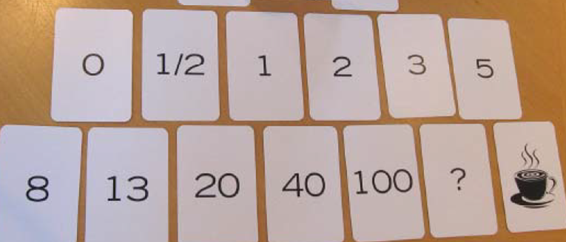
\includegraphics[width=0.7\textwidth]{planningPoker}
 		\caption{Planning poker}
	\end{figure}
	
 	\item Diferencia entre historia y tarea
 	
 	La diferencia es simple, la primera es aquello que se le entrega al dueño del producto; la segunda, los archivos no entregables o aspectos que no preocupan al dueño del proyecto.
 	
 	\item Definir sitio y hora para el \textit{scrum} diario
 	
 	El primer \textit{scrum} es el lanzamiento, cuando decide el personal por dónde empezará a trabajar. Existen dos formas de reuniones:
 	
 	\underline{Por la mañana}, consiste en recordar lo que se realizo el día anterior para ponerlo en común y acordar la tarea a realizar hoy y \underline{por la tarde}, consiste en recordar lo que hemos realizaste durante la jornada de trabajo y hablar sobre lo que realizaras el día de mañana.
 	
 	\item Historias no funcionales
 	
 	Son elementos no funcionales, es decir, son los archivos o elementos no entregables o que no están relacionadas con ninguna historia específica y no tienen mucho valor para el dueño del producto. 
 	
 	Por ejemplo: escribir una descripción del diseño, refactorizar los accesos a los datos o tener un seguimiento de los errores o programa encargado de ello.
	
	\item Seguimiento de errores vs. pila del producto
	
	Hay diferentes programas para el seguimiento de errores. En el libro recomiendan (\textit{Jira}), ya que Excel es un formato bueno para la pila de producto, pero no es tan específico para los errores.
	
	\item Finaliza la planificación del \textit{sprint}
	
	La reunión llega a su fin cuando el dueño del producto y los miembros del equipo llegan a consenso. Una vez que están todos de de acuerdo, el siguiente paso es comenzar a trabajar con un \textit{scrum} diariamente durante las siguientes semanas de trabajo.
\end{enumerate}

\section{Cómo comunicamos los \textit{sprint}}

La comunicación entre la plantilla de trabajo es crucial a la hora de informar sobre lo que está ocurriendo en cada jornada de trabajo. Para informar en todo momento de lo que está sucediendo, en el libro indican que puede ser beneficioso crear una página de información del \textit{sprint}, donde se indiquen los objetivos, pasos a cumplir y fechas de entrega. El jefe del \textit{scrum} podrá imprimir la hoja y dejarla en un lugar visible para que todos los
miembros puedan saber dónde está el \textit{sprint} actualmente.

\section{Cómo hacemos las pilas de \textit{sprint}}

Una vez haya concluido la reunión de planificación del \textit{sprint} y se haya informado a los trabajadores de ello, el jefe del proyecto (\textit{scrum Máster}) debe crear una pila de \textit{sprint}. Esto se hace antes de la reunión de planificación de \textit{sprint}, pero antes del primer \textit{scrum} diario.

El formato de la pila será una lista de tareas, como la imagen que se muestra
a continuación:

\imagen{TablonTareas}{Tablón de tareas}

En dicha tabla se podrán añadir todas las columnas que se deseen, por ejemplo: Test funcionando, proceso cancelado, etc.

El diagrama \textit{burn-down} indicara cómo va el proyecto con respecto al tiempo empleado. (trabajo restante/ fecha estimada).

El gráfico \textit{burn-down} puede indicar varios síntomas:
\begin{itemize}
	\item \underline{Alarmante}: cuando la línea está por encima de la línea de puntos, se considerará quitar elementos de la pila del \textit{sprint}.
	\item \underline{Buen camino}: cuando la línea está por debajo de la línea de puntos, se considerará añadir nuevas historias al \textit{sprint}.
	
\end{itemize}

El \textit{Scrum Máster} es el responsable de asegurarse de que el equipo actúa ante diferentes señales como que se acumulen las actividades en la tarea pendiente o el gráfico \textit{burn-down} no siga una tendencia recta.

\section{Cómo distribuimos la sala del equipo}

Los miembros se reúnen en frente de una pizarra para que se puedan observar entre ellos mientras exponen ideas de cómo abordar los diferentes errores o ideas que puedan surgir durante el devenir del proyecto.

También es importante que los miembros del equipo se sienten juntos o cercanos en el área de trabajo para fomentar la comunicación entre ellos. 

Ventajas de trabajar juntos en la oficina \underline{resultados inmediatos}, \underline{audibilidad} posibilidad de hablar con cualquier miembro del equipo sin levantarse de la silla, \underline{visibilidad} todos los trabajadores pueden ver lo que sucede y tener cercano el tablón de tareas y \underline{aislamiento} mayor orden a la hora de reunir al equipo y no tener que levantarse y molestar a molestar al resto de compañeros de la oficina.

Si el equipo está distribuido, se intentará que este lo más cercano posible usando técnicas como videoconferencia, \textit{webcams}, maquinas remotas de escritorio, etc.

Sería recomendable que el dueño del producto esté cerca para consultar dudas y el tablón de tareas, pero no lo suficientemente cerca de estar al lado del equipo, ya que puede que no sea capaz de controlarse y pueda interrumpir en cualquier detalle y provocar que el equipo no fluya adecuadamente.

\section{Cómo hacemos los \textit{scrums} diarios}

Deben ser realizados todos los días, a la misma hora y en el mismo lugar. Se suelen realizar de pie para intentar que no sobrepasen los 15 minutos de duración. Una vez realizado el \textit{scrum}, actualizamos el tablón de tareas de acuerdo con las indicaciones de los trabajadores sobre lo que realizaron el día anterior y los planes que tienen para ese día. Lo puede realizar el \textit{Scrum Máster} y así, mientras los trabajadores lo indican, él va modificando los \textit{post-it} en el tablón, para incentivar que la gente no llegue tarde, en el libro recomienda el uso de pequeñas multas para que no haya informales en el grupo de trabajo.

\section{Cómo hacemos la \textit{demo} de \textit{\textit{sprint}}}

Tener que hacer una demostración con cada final del \textit{sprint} obliga al equipo a poder demostrar el trabajo realizado durante ese proceso, esto es favorable ya que consigue un \textit{feedback} entre las partes interesadas en el proyecto. Con esto se intenta conseguir un reconocimiento a los trabajadores y las personas que no son parte del proyecto sea capaz de entender lo que realiza el equipo si las demostraciones son claras y descriptivas, estaremos consiguiendo un ahorro de trabajo para futuro trabajo.

\section{Cómo hacemos las retrospectivas de \textit{sprint}}

Las retrospectivas son importantes, en vista de que con ello conseguimos y nos aseguramos de que son realizadas por el equipo. Permite, además, mejorar ideas o alguna cosa que el grupo vio mal en el anterior \textit{sprint}, con el objetivo de que no se vuelva a repetir de nuevo en los posteriores \textit{sprint}.

El autor indica un ejemplo para realizar las retrospectivas:

\begin{itemize}
	\item Reservar de una a tres horas, dependiendo la discusión.
	\item Los representantes: el dueño del producto y el equipo.
	\item Intentar que sea una reunión cómoda y sin gente interrumpiendo.
	\item Designar un secretario.
	\item Intentar que participe todo el mundo, opiniones, errores e ideas sobre el próximo \textit{sprint}.
	\item Observar los tiempos reales con los que teníamos estimados.
\end{itemize}

Se puede escribir sobre una pizarra las retrospectivas con tres columnas: \textbf{buena}, si volviéramos a realizar esta tarea, realizaríamos los mismos pasos, \textbf{mejorable}, ¿qué cambiaríamos si lo volveríamos a realizar las mismas personas? y \textbf{mejoras}, ideas concretas sobre qué mejorar en el futuro.

Se podría decir que \textit{bien} y \textit{mejorable} son miradas al pasado y \textit{mejoras}, miradas al futuro.

\section{Descansos entre \textit{sprint}}

Como indica el libro, no se puede estar siempre esprintando ya que acabarías derrotado y al final estarías haciendo \textit{footing}.

Los \textit{sprint} son muy intensos y por ello hay que dejar espacio entre ellos. Con esto se consigue liberar la cabeza y, \textit{a posteriori}, aportar mejores ideas.

Es conveniente que la retrospectiva y la siguiente reunión no tengan lugar en el mismo día y es incluso aconsejable realizarla con el fin de semana de por medio.

Un de las mejores ideas que propone es tener un día de laboratorio (que los trabajadores puedan tener momentos largos de libertad) para poder realizar otras cosas relacionadas con el trabajo, pero no con ese trabajo, esta idea está inspirada en Google.

%\imagen{DescansosEntreSprint}{Descansos entre \textit{sprint}}

Lo más importante es que entre \textit{sprint} y \textit{sprint} haya horas de desconexión y te permitan dormir para relajarte.

\section{Planificación de entregas y los contratos de precio fijo}

En algunas ocasiones, cuando el contrato es de precio cerrado, necesitamos planificar los \textit{sprint} con antelación. Por ello el propietario necesita las estimaciones aproximadas de las tareas que se incluirán en el contrato, estas tareas las deberá haber realizado con antelación el equipo de trabajo. 

\subsection{Definir los umbrales de aceptación y estimar elementos importantes}

Los umbrales son una clasificación según la importancia de la pila de producto de acuerdo con los términos que aparezcan en el contrato. Conforme con dónde esté el umbral de aceptación, meteremos esto en las diferentes versiones de nuestro proyecto.

Para estimar los elementos más importantes, se deben incluir todas las historias que se añaden en el contrato. Las estimaciones las tendrá que realizar el equipo y no tendrá que dedicarse demasiado tiempo para ello, son estimaciones no compromisos.

\imagen{estimacionElementos}{Estimación de los elementos}

Después de realizar cada \textit{sprint} comprobaremos la velocidad real del \textit{sprint} y, en caso de que sea muy diferente a la que se estimó en un principio, revisaremos la velocidad que dijimos en el resto del \textit{sprint} y tendremos que actualizar el plan de entregas. Quizás la modificación de las entregas no guste al cliente, pero lo que se intenta es cumplir el objetivo y ser honestos con él.

\section{Cómo combinamos \textit{Scrum} con XP}

Hay que indicar que tanto \textit{scrum} como XP (Programación eXtrema) se combinan de forma perfecta, dado que \textit{scrum} se centra en prácticas de organización y gestión, mientras que XP se centra en prácticas de programación. Ya que tratan áreas diferentes pueden complementarse muy bien entre ellas.

Los beneficios de la programación por parejas son:

Mejorar la calidad del código, la concentración, la distribución del conocimiento entre el equipo, poder cambiar de parejas para aportar nuevas ideas, poder estandarizar el código(esto puede ser útil si se cambia de parejas).

El desarrollo guiado por pruebas TDD es un test automático, en el cual tú escribes el código necesario para pasar ese test y a continuación refactorizas el cogido para su legibilidad y eliminar posibles duplicaciones.

TDD es duro, puede llevar tiempo comprenderlo, pero es muy importante, tiene efecto positivo en el diseño del sistema además tiene pruebas de integración tipo ``caja negra'' y permite utilizarlo con otros programas como \textit{Jetty}, Cobertura (métricas).

Una parte importante es el diseño incremental. Consiste en mantener el diseño simple desde el momento que empezamos el proyecto e ir mejorándolo continuamente, posteriormente se podrá limpiar el código y revisarlo. Primeramente, es necesario que funcione de forma correcta, las mejoras del diseño son efectos del realizar el TDD.

Es importante la integración continua, con esto evitamos el problema de que el proyecto funcione en todas las maquinas. Una vez compilado en un ordenador, realizamos la copia en otro servidor y este se encarga de comprobar el funcionamiento y correr con todas las pruebas. El entorno que recomiendan es el basado en \textit{Maven} y \textit{QuickBuild}.

\section{Cómo hacemos pruebas}

Posiblemente es la parte más dura del \textit{scrum} ya que la realización de estas puede resultar la parte más variable entre las diferentes organizaciones. 

Nada está acabado hasta que el equipo de pruebas lo da por finalizado. Si por un casual el equipo destinado a las pruebas no está trabajando en un momento dado, lo óptimo sería que vaya preparando las pruebas para así adelantar trabajo.

\imagen{ejecutarPruebas}{Ejecución del orden de las pruebas}

Para minimizar la fase de pruebas se puede reducir la cantidad de tiempo que se dedica a este proceso. Esto se consigue de dos formas: maximizando la calidad del código desarrollado por el equipo o maximizando la eficiencia del trabajo manual de pruebas (\textit{beta-tester} y dándoles  mejores herramientas).

Para incrementar la calidad se puede incluir a un miembro del equipo de las pruebas en el equipo \textit{scrum}, con esto podríamos cumplir los tiempos ya que los \textit{sprint} tienen un tiempo limitado. De esta manera, se podría optimizar el tiempo y conseguir los objetivos.

Si todo fuera perfecto,  veríamos innecesario el papel del equipo de pruebas ya que cada equipo \textit{scrum} entregaría la versión directa para salir al mercado tras cada \textit{sprint}. Pero esto no suele acontecer así ya que al finalizar el \textit{sprint} uno y pasar al dos, seguramente nos encontremos con algún error en el código. Por esa razón los equipos de prueba son tan necesarios.

\section{Cómo manejar múltiples equipos \textit{Scrum}}

Cuando tienes varios equipos trabajando en un mismo proyecto, la cosa se puede complicar y esto te genera una serie de preguntas: cuántos equipos crear y cómo distribuirlos.

Cuanta más gente en el mismo \textit{scrum} tiende a ser un conflicto mayor ya que los \textit{scrum} diarios tienden a durar más que los 15 minutos que se estipularon en un principio y puede que los miembros del equipo no sepan lo que hacen otros, y esto puede crear confusión.

Lo aconsejable en este caso es dividir los equipos en equipos entre 5 y 9 personas.

\subsection{¿Los \textit{sprint} deben ser sincronizados o no?}

Suponiendo que tenemos a más de un equipo \textit{scrum} trabajando en el mismo producto, nos plantemos la idea de que si se tendría que tener los \textit{sprint} sincronizados. Esto quiere decir, ¿se tendrían que empezar y acabar al mismo tiempo o, por el contrario, deberían solaparse?

Si lo realizábamos de forma solapada siempre tendríamos un \textit{sprint} cercano a finalizar y otro  recién comenzado, lo que implicaría que habría entregas constantes y la carga del dueño del producto podría distribuirse en el tiempo de forma equitativa (Ilustración 3.10).

\imagen{tiempoSolapado}{Tiempo solapado}

Pero viendo los \textit{sprint} sincronizados el autor del libro se dio cuenta que todos los equipos podrían trabajar en el mismo \textit{sprint} y realizar las reuniones correspondientes para una mejor planificación; se lograría también se lograría una menor sobrecarga y se realizarían menos reuniones de planificaciones y \textit{demos}.

\imagen{tiempoSincronizado}{Tiempo sincronizado}

\section{Asignación y distribución de las personas en los equipos}

Hay dos estrategias para la asignación de las personas a los equipos cuando hay varios para el mismo producto. Los podrá crear el dueño o bien los trabajadores del proyecto. Lo óptimo sería crear equipos multifuncionales, es decir, que sepan desenvolverse en varios ámbitos. Por otra parte, no es recomendable tener miembros en el equipo a tiempo parcial.

También se realizan \textit{scrum} de \textit{scrums} donde los jefes de cada \textit{scrum} se reúnen periódicamente para y analizar cómo va el avance, aclarar las posibles dudas que puedan surgir y estudiar los siguientes puntos a tratar antes de celebrar la próxima reunión. 

En cuanto a la distribución siempre intentaremos acercar el ancho de banda de la comunicación entre los miembros del equipo separados. Se intenta programar por parejas, así conseguimos que las personas socialicen, intentar realizar el \textit{scrum} diario y intentar que tengan la misma versión de la pila, para tener los datos sincronizados.

	Los métodos más comunes para la comunciación son webcam, salas de runiones, salaz zoom, programas de intercambio express, etc

\subsection{\textit{Offshoring}}

Al tener varios equipos en diferentes localizaciones, se recomiendan tres opciones para intentar gestionar la situación eficientemente utilizando \textit{scrum}.

\begin{enumerate}[1.]
	\item Equipos separados: los miembros del equipo no-equipo conjunto de \textit{scrum} trabajan independientemente de la localización y simplemente intentaran sacar la producción de cada uno de los objetivos que se van marcando.

	\item Miembros de equipos separados: se intenta que se conozcan entre sí todos los miembros del equipo y también tener un método de comunicación adecuado entre las dos localizaciones. Se persigue que los equipos sean pequeños para intentar formar un solo equipo \textit{scrum} (independientemente de las localizaciones).
		
	\item También se puede dar el caso que haya gente trabajando desde casa por diferentes motivos, este es el caso mas positivo ya que están cerca de la oficina y se puede intentar llegar a acuerdos para que algún día trabaje desde la oficina.
\end{enumerate}

\section{Lista de comprobación del \textit{Scrum Máster}}

En este último capítulo se realizan las comprobaciones de las rutinas de los \textit{Scrum Máster} se enumerarán todas las cosas que son susceptibles a olvidar.

\textbf{Comienzo del \textit{sprint}}: se realiza una planificación del \textit{sprint}, se anuncia mediante correo electrónico el comienzo de un nuevo \textit{sprint} y se actualizar el documento de estadísticas donde se añaden las velocidades estimadas.

\textbf{Todos los días}: nos aseguramos en el comienzo del \textit{sprint} diario que se incluyen todas las historias de la pila, notificaremos al dueño del producto todos los cambios que se comentan, mantenemos la pila y el \textit{burn-down} siempre actualizados y intentaremos solucionar todo tipo de problemas y si no, informar al dueño o al jefe de desarrollo.

\textbf{Final del \textit{sprint}}: realizamos la\textit{demo} de \textit{sprint}, informamos a toda la gente de la realización de la \textit{demo} con antelación, realizamos una retrospectiva de  \textit{sprint} con el equipo y el dueño del producto y actualizamos el cuaderno de estadísticas de  \textit{sprint}, en el cual incluimos la velocidad real y los puntos clave de la retrospectiva

\newpage
\capitulo{3}{Conceptos teóricos \textit{Blockchain}}
Una vez acabado el libro, ``\textit{Scrum y XP desde las trincheras}'', el siguiente paso en la realización del proyecto es el estudio y la creación de la tecnología \textit{blockchain}. Estuvimos observando los puntos más importantes para empezar con el guion e intentar realizar una web que fuera útil para nuestro proyecto. 

A continuación, hablaremos sobre dicha tecnología: 

\section{Origen del \textit{blockchain}}

En 1997, hace ahora 21 años, Adam Back inventó \textit{hashcash}, cuyo primer uso era para combatir el correo basura o \textit{spam}, pero actualmente se conoce más por el uso en Bitcoin\cite{bitcoin}\cite{bitcoin1}.

\textit{Hashcash}\cite{wiki:HashCash} es una tecnología de prueba de trabajo o \textit{proof of work (POW)} cuya estrategia es establecer un algoritmo que requiere un trabajo de computación para demostrar la verificación de quién manda el mensaje. Tiene mucho interés ya que, para mandar mensajes, tienes que estar dispuesto a realizar un pago por el medio de trabajo de la \textit{CPU}(Unidad Central de Procesamiento), de esta forma si quieres mandar grandes cantidades de correo basura, tendrían que dedicar mucho tiempo en el en el rendimiento de la \textit{CPU}.


En octubre de 2008 Satoshi Nakamoto publicó Bitcoin P2P \textit{e-cash}, un sistema \textit{peer-to-peer} de dinero electrónico sin intermediarios financieros ni de ningún tipo. 

El 3 de enero de 2009 tuvo lugar el primer bloque de la \textit{blockchain} de Bitcoin.

\section{Que es \textit{blockchain}}
\textit{Blockchain}\cite{blockcahin} es un almacén de datos distribuidos. Este sistema crea copias en lo que se llama el libro mayor, esto significa que tiene una especie de registros digitales en la cual introducimos información y una vez esta es introducida, está ya no podrá ser borrada. Esta información se almacena en miles y millones de computadoras, también llamadas nodos. Un número razonable de nodos debe validar cada nuevo registro antes de que sea registrado. Una vez confirmado, el registro se almacena en el libro mayor y se propaga a través de la red de nodos participantes. En esta tecnología para poder añadir nueva información, se tiene que añadir bajo el acuerdo de todos los nodos.
 
Los contratos inteligentes, programas que se ejecutan automáticamente en el \textit{blockchain} después de la finalización de la transacción, amplían aun más las capacidades de la tecnología. Los contratos inteligentes permiten el desarrollo de organizaciones autónomas y empresas que se pueden gestionar a través del consenso y el control de la multitud.

\textit{Blockchain} es la descentralización en su expresión tecnológica. En vez de una autoridad central que adopte las decisiones y reglas de juego, los datos (criptomonedas, información, contratos, etc.) se transfieren, validan o almacenan de forma distribuida a lo largo de muchas redes de computadoras tendidas en diferentes partes del mundo sin ninguna jerarquía entre sí.

En el escenario que se trabaja bajo la cadena de bloques o \textit{blockchain}  aparecen:
\begin{enumerate}
	\item \underline{Los bloques}: conjunto de transacciones e información de la cadena. Están compuestos por un código numérico, el código del paquete a tratar y otro código numérico. 
	\item \underline{Mineros}: son los ordenadores que permite la potencia computacional.
	\item \underline{Nodos}: son los ordenadores que almacenan y distribuyen la copia actualizada.
\end{enumerate}

La cadena de bloque es una red P2P\footnote{\textit{Red peer-to-peer}: es una red de ordenadores en la cual estos actúan simultáneamente como clientes y servidores respecto a los demás nodos de la red. Permite el intercambio de información entre los ordenadores que estén interconectados.}(red peer-to-peer) en la cual cada ordenador tiene la misma importancia.


\imagen{redP2P}{Red Peer-to-Peer}

\section{Proyectos que usan \textit{blockchain}.}

Hay muchos proyectos que usan blockchain, pero aquí destacaremos el uso de tres proyectos que se enfocan principalmente en esta tecnología \textit{Bitcoin}, \textit{Ethereum} y \textit{Hyperledger}.
\section{\textit{Bitcoin}}
\subsection{Origen de \textit{Bitcoin}}

El origen del \textit{Bitcoin} se da en 2007, el creador es: Satoshi Nakamoto y él originó este sistema de pagos electrónicos basado en pruebas criptográficas en vez de confianza, permitiendo que dos partes interesadas realicen transacciones directamente sin la necesidad de una tercera parte confiable. Este sistema dio origen a la criptomoneda \textit{Bitcoin} y la tecnología con la que opera se denominó \textit{blockchain} o cadena de bloques. 

Bitcoin surge como una solución a la necesidad de los usuarios de un intercambio mundial facilitado por herramientas de pago transaccionalmente y que, a menudo, se traduce en la voluntad de no tener que emplear la moneda o los billetes.

\imagen{bitcoin}{Moneda Bitcoin}

\subsection{Para qué sirve Bitcoin}

Bitcoin es una moneda, como el euro o el dólar estadounidense, que sirve para intercambiar bienes y servicios. 
La diferencia con otras monedas es que \textit{Bitcoin} es una divisa electrónica que presenta novedosas características y destaca por su eficiencia, seguridad y facilidad de intercambio.
Su mayor diferencia frente al resto de monedas se trata de una moneda que nadie la controla(descentralizada). 
La idea, plasmada en un \textit{white paper} era crear un sistema de intercambio de efectivo electrónico P2P (\textit{peer-to-peer}) que no pasara por instituciones financieras tradicionales. 

\subsection{Proceso de extracción}

\subsubsection{\textit{Proof of work} o prueba de trabajo}
La prueba de trabajo\cite{pow} es un proceso que nace con el objetivo de eliminar los ataques a redes informáticas a través de la realización de una prueba moderadamente difícil (ej. demostrar que no eres un robot) es una especie de \textit{captcha}\footnote{Es un test de Turing público y automático para distinguir a los ordenadores de los humanos, sirve de medida de seguridad conocido como autenticación pregunta-respuesta.} para poder permitir la realización de la acción que se desee.

Este algoritmo es usado para realizar las transacciones y poder obtener o producir nuevos bloques en la cadena. Con esto se consigue que los mineros compiten entre ellos para completar transacciones en la red y obtener recompensas.

La implementación de este algoritmo es un pequeño pequeño rompecabezas que depende de varios factores: 
\begin{itemize}
	\item Cantidad de usuarios.
	\item Potencia actual del equipo
	\item Carga que soporta la red.
\end{itemize}

Como dato, sabemos que el \textit{hash} de cada bloque contiene el \textit{hash} del bloque anterior, esto lo que nos garantiza es que tiene mayor seguridad y evita la posible violación del bloque.

\imagen{pow}{Prueba de trabajo}

El tiempo medio de la formación de bloque es de diez minutos.

\subsubsection{\textit{Proof of stake} o prueba de participación}

La prueba de participación\cite{pos} es un protocolo de consenso\footnote{\underline{Protocolo de consenso}: encontramos un problema ya que consiste en poner de acuerdo a múltiples procesos en una cosa conjunta. Cuantos menos fallos más fácil llegar a consenso, pero habitualmente la solución a estos problemas suele ser un algoritmo o algún tipo de protocolo antes establecido, esto siempre suele ser usado por los procesos que no tienen intenciones maliciosas.} que asegura una red de posesión de monedas. Con este sistema, las opciones de encontrar un bloque de transacciones y recibir monedas son proporcional a la cantidad de monedas que tenemos almacenadas en nuestra cuenta.

Tenemos diferentes estrategias desarrolladas en forma de algoritmo:

\begin{itemize}
	\item \underline{Prueba de participación pura}: este algoritmo consiste en la creación de bloques mas fáciles para los que controlan gran cantidad de monedas. 
	\item \underline{Prueba de deposito o \textit{proof of deposit}}: este algoritmo esta enfocado al momento en el que las monedas son usadas por el dueño del bloque y crear otros nuevos. Estas son congeladas hasta que se confirme un número determinado de bloques. Aquí no se recompensa a un minero por almacenar monedas no gastadas en el pasado, se recompensa a los que están dispuestos a tener monedas inmóviles durante un gran periodo de tiempo.
\end{itemize}

\subsection{Dinero electrónico}

Un \textit{Bitcoin} no es más que una cadena de caracteres que está vinculada en un momento a una cartera. 
Un usuario crea una cartera, que contiene una dirección pública, la cual es anónima, y dicha cartera tendrá almacenadas las criptomonedas similar al funcionamiento de un banco electrónico. Esa dirección puede compartirse para recibir pagos.
Toda transacción entre \textit{wallets} queda registrada en el blockchain, la médula espinal de las criptomonedas. El \textit{blockchain} registra todas las transacciones de esta moneda virtual que se han completado desde la creación de la cartera.

La divisa ahora mismo "a fecha de 09/04/2019" es: 1 Bitcoin equivale a 7.233,81 \euro

\section{\textit{Ethereum}}
\subsection{Origen de \textit{Ethereum}}

En el 2014, surge Ethereum\cite{ethereum} de manos de Vitalik Buterin de origen ruso. Se trata de un investigador y programador de criptomonedas. 

El desarrollo de \textit{Ethereum} empezó siendo financiado por un \textit{crowdsale}\footnote{\textit{Crowdfunding}\cite{crowdfunding}: práctica para financiar proyetos al recaudar por medio de Internet pequeñas cantidades de dinero de un gran número de personas.}

A mediados de 2015, se crearon 72 millones de monedas \textit{Ether}, y actualmente esta cifra representa sobre le 70\% del total de Ether mundial.
 
\subsection{Para qué sirve \textit{Ethereum}}

\textit{Ethereum}\cite{ethereum1} es una plataforma \textit{open source}\footnote{\textit{Plataforma source}: programas informáticos que permiten el acceso a su código de programación, lo que facilita modificaciones por parte de otros programadores ajenos a los creadores originales }, descentralizada que permite la creación de acuerdos de contratos inteligentes entre pares, basada en el modelo \textit{blockchain}.
Cualquier desarrollador puede crear y publicar aplicaciones distribuidas que realicen contratos inteligentes. 
\textit{Ethereum} también provee una ficha de criptomoneda que se llama \textit{Ether}.
Se puede intercambiar \textit{Ether} entre cuentas diferentes y también es utilizado para compensar los nodos participantes por los cálculos realizados.

El \textit{Ether} es la criptomoneda de \textit{Ethereum}.

La divisa ahora mismo "a fecha de 09/04/2019" es: 1 \textit{Ether}  equivale a 146,95\euro.

\subsection{Ventajas del \textit{Ether}}

Las principales ventajas del \textit{Ether}, con respecto a las monedas tradicionales, son similares a las otras criptomonedas y parecidas a al \textit{Bitcoin}, y se pueden resumir en:
\begin{itemize}
 	\item No las controla ningún gobierno y no se puede contar su valor. 
	\item Son más difíciles de falsificar que las monedas tradicionales \euro, \$, \pounds, etc
	\item No existen intermediarios cuando se realizan transacciones o pagos y esto hace que sea más barato el realizarlas.
	\item El sistema de código es abierto, por lo tanto, permite realizar mejoras, como nos pasa con el Bitcoin.
\end{itemize}

\subsection{¿Qué es el Gas?}

El Gas\cite{gas} es un proceso de pago que tiene como obligación establecer un determinado número de ejecuciones computacionales. Con esto lo que evitamos es fomentar los bucles infinitos y cualquier otro desperdicio en el código.

El Gas persigue el objetivo final de controlar los precios de las transacciones. Al mismo tiempo, sirve para reducir los \textit{spam} y poder asignar recursos en la red.

La meta es que cada usuario pague una comisión por los recursos que consume. Aquí se incluye el ancho de banda, la computación y el almacenamiento. Por ello, al realizar una operación que consuma unos recursos tendrá una comisión proporcional al uso que haga de esta.

\section{\textit{Hyperledger}}

\subsection{Origen de \textit{Hyperledger}}

El origen se sitúa en diciembre de 2015 y fue creado por la Fundación \textit{Linux}, es una plataforma código abierto para \textit{blockchain}, para apoyar a los \textit{ledgers} distribuidos basados en la \textit{blockchain}.

Es una plataforma privada de \textit{Blockchain}. Es una colaboración global entre empresas y expertos para facilitar y mejorar la adopción de la cadena de bloques entre ellas.

\subsection{Proyectos de \textit{Hyperledger}}

Actualmente en \textit{Hyperledger}\cite{hyperledger} se encuentran nueve proyectos, los cuales se pueden dividir en dos ramas principales: 

\begin{enumerate}

	\item Plataformas \textit{blockchain}
	
	\begin{enumerate}[1)]
		\item Hyperledger Burrow: impulsada por la \textit{startup} Monax Industries y es una \textit{blockchain} privada basada en código de Ethereum. Permite el despliegue de \textit{smart contract} dados en Solidity.
	\item Hyperledger Fabric: es el proyecto mas conocido de Hyperledger. Orientado al mundo de empresas (IBM). Intenta facilitar la implementación en la plataforma multidisciplinar de cualquier modelo de uso. Permite el uso de Smart-contracts (\textit{chaincodes}). 
Es flexible, incorpora como crear \textit{chaincodes} en cualquier lenguaje.
	\item Hyperledger Indy: propone una solución a la identidad digital. Intenta que los datos tengan que ser gestionados por cada usuario. Procura no dar información a terceras personas.
	\item Hyperledger Iroha: quiere ser una \textit{blockchain} simple y modularizada que permita los \textit{smart contract} desarrollados en Java, y pretende conseguir el menor uso de los datos personales. 
	\item Hyperledger Sawtooth: viene de Intel, una \textit{blockchain} privada con uso empresarial que incorpora el despliegue de \textit{smart contract}. También se desarrolla en Solidity. 
\end{enumerate} 
	\item Herramientas para la interacción con las plataformas
	\begin{enumerate}[1)]
		\item Hyperledger Composer: permite la creación de aplicaciones descentralizadas.
		\item Hyperledger Explorer: intenta dar una interfaz para la monitorización de los nodos (\textit{peers}) de Hyperledger Fabric. Tiene un servicio para la comunicación de \textit{Blockchain} y la aplicación. 
		\item Hyperledger Cello: crea una solución que consiga un modelo de despliegue, ``\textit{blockchain} como Servicio''. Reduce el esfuerzo de crear una infraestructura de nodos \textit{blockchain}.
		\item Hyperledger Quilt: el objetivo es la conexión entre distintas redes de \textit{blockchain} mediante el protocolo Interledger (ILP). El protocolo intenta quitar los pagos entre distintos sistemas bancario. ILP permite realizar transferencias entre distintos “\textit{ledgers}” (libro de cuentas) y permite la conexión de usuarios con las cuentas que tienen en distintos sistemas.
	\end{enumerate}
\end{enumerate}

\section{Plataforma de desarrollo: Solidity y D'app}

\subsection{Solidity}

Solidity\cite{solidity} es un lenguaje de alto nivel orientado a contratos. Su sintaxis es similar a la de \textit{JavaScript} y está enfocado, específicamente, a la Máquina Virtual de Ethereum\footnote{EVM: software que interactúa con la red de Ethereum y permite ala creación de aplicaciones independientemente del lenguaje de programación usado.} (EVM).

En el ámbito de Solidity\cite{solidity1}, los desarrolladores pueden escribir aplicaciones descentralizadas que se puedan implementar en automatizaciones de negocios mediante contratos inteligentes. Esto dejará un registro autorizado y con pruebas demostrables de los pasos realizados. En solidity tendremos una serie de modificadores, gracias a los cuales podremos pedir una cantidad de pago concreta o que la transacción tenga herencia, o una operación solamente la pueda realizar un usuario concreto, habrá posibilidad de crear arrays, eventos, funciones privadas, al ser un lenguaje actual y nuevo para nosotros, la información no era tan clara y abundante como en otros lenguajes.

Al decir que es un lenguaje de alto nivel nos referimos a un lenguaje de \textit{Turing Complete}, este concepto fue creado por \textit{Alan Turing}, y cuando se aplica a la tecnología \textit{blockchain} se refiere a la capacidad de un lenguaje para poder resolver cualquier problema de computo y poder añadir nuevas reglas, como serían los bucles\footnote{Bucle: una instrucción repetitiva para poder ejecutar los problemas.}.

\subsection{Construir sobre \textit{Ethereum}}

Las principales razones por la cual las \textit{DApp} se construyen sobre Ethereum en vez de ser independientes son:
\begin{itemize}
	\item Seguridad:  construir esa \textit{DApp} basada en \textit{Ethereum} hará que sea la gran red de nodos de Ethereum la que procesen sus transacciones, aumentando exponencialmente su seguridad.
	
	\item Interoperabilidad: Están escritas en el mismo lenguaje (\textit{Solidity}), por lo que todos los programadores que  los programadores que lo conozcan lo saben interpretar, se pueden utilizar las transacciones y se pueden utilizar las unas con las otras (puede haber sinergias)
\end{itemize}

\subsection{\textit{DApp}}

Herramienta de construcción, gestión de paquetes y asistente de despliegue para Solidity.

Las \textit{DApp}\cite{dapp}\cite{dapp1} son código \textit{back-end}\footnote{\textit{Back-end}: es el que se encuentra en la parte del servidor(PHP, Python, Java) e interactúa con la base de datos verificando usuarios y montando la página}, el cual se ejecuta sobre la red P2P (\textit{peer-to-peer}).

Son aplicaciones distribuidas que interactúan directamente con \textit{blockchain}.

Con el uso de las DApp se permite descentralizar el código \textit{Back-end} y los datos, esto quiere decir que son inmutables, no se pueden falsificar y solamente depende de la comunidad de usuarios que la utilizan. 

La aplicación descentralizada puede ser una aplicación móvil o una aplicación web que interactúa con un contrato inteligente para llevar a cabo su función.

\subsubsection{Condiciones de una DApp}

Las características que definen a una DApp son las siguientes:

\begin{enumerate}
	\item Aplicación totalmente de código abierto, debe operar de forma autónoma, sin nadie que este controlando. Se pueden aplicar cambios, pero todos ellos tiene que ser decididos por consenso entre los usuarios.
	\item Los datos de cada operación son almacenados en una \textit{blockchain} pública y descentralizada.
	\item La aplicación tendrá una ficha, la cual es necesaria para acceder y recompensar a los mineros que trabajen sobre dicha aplicación.
	\item La propia aplicación generará fichas, dependiendo del algoritmo, para tener una prueba de su valor.
	 
\end{enumerate}

\subsection{Tipos de \textit{DApp}}

\begin{enumerate}
	\item \underline{Tipo I}: estas son las que tendrían su propia cadena de bloques independiente. Podría ser el equivalente a un sistema operativo de un ordenador.
	\item \underline{Tipo II}: utilizan la \textit{blockchain} de una aplicación descentralizada tipo I en vez de tener ellas una propia. Este tipo de DApp son protocolos que funcionan ya sea con sus propios tokens o con los \textit{tokens} de la \textit{blockchain} en la que operan. Ej: raiden network. Sería el equivalente a un programa con un propósito general, véase un Word o Excel.
	\item \underline{Tipo III}: utilizan el protocolo de una aplicación descentralizada de tipo II. Sería lo mismo que una solución de software especializada para ese procesador de texto, como un plugin o herramienta que añada servicios al Word, Excel o Dropbox. 
\end{enumerate}

\section{\textit{Smart contracts}}

Los \textit{smart contracts} tienen como objetivo eliminar intermediarios con el objetivo de simplificar los procesos para ahorrar costes al consumidor.

\subsection{¿Qué es un \textit{smart contract}?}

Un \textit{smart contract}\cite{smartContract}\cite{smartContract1} o contrato inteligente es similar a un contrato y no es más que un acuerdo entre dos o más implicados con unas reglas que tendrán que aceptar todas las partes para, así, entender los objetivos a cumplir. 

Anteriormente los contratos se cerraban de forma verbal o mediante documentos escritos, en cambio, en los contratos inteligentes son capaces de ejecutarse y poder cumplirse mediante ellos mismos, de una forma automática y autónoma, sin la necesidad de ningún intermediario o notario. 

Los \textit{smart contract} son unos \textit{scripts} \footnote{\textit{Script}: es un documento que contiene instrucciones, escritas en códigos de programación.} que, a la vez, son los términos del contrato. Los \textit{smart contract} tienen una validez total sin depender de nadie ya que es un visible por todos y no se puede cambiar al existir sobre la tecnología \textit{blockchain}, que es la causante del carácter descentralizado, inmutable y transparente.

\subsection{Ventajas de los \textit{smart contracts}}

Las principales ventajas de estos contratos son: 

\begin{itemize}
	\item \underline{Autonomía}: no se necesita ningún intermediario ya que tú realizas el acuerdo y con esto esto se evita el problema de la manipulación de terceras personas
	\item \underline{Confianza}: los documentos están encriptados y no hay manera de qué se pueda decir que se perdió. 
	\item \underline{Respaldo}: los documentos son guardados en varios ordenadores, por lo que con esta cadena de bloques estás bien cubierto ante la posibilidad de perdida.
	\item \underline{Seguridad}: gracias a la criptografía, los documentos se mantienen a salvo y no esta la posibilidad de que se realicen \textit{hackeos}. 
	\item \underline{Velocidad}: gracias a los contratos inteligentes podemos reducir notoriamente el tiempo empleado estos también utilizan un código de \textit{software} que consigue automatizar las tareas y ahorrar tiempo. 
	\item \underline{Ahorros}: gracias a este tipo de contrato conseguimos ahorrar mucho dinero ya que que eliminamos la presencia de uno o varios intermediarios. 
	\item \underline{Precisión}: estos contratos son muy rápidos, económicos y evitan los errores de rellenar formularios.
\end{itemize}

Se podría decir que gracias estos contratos inteligentes se puede garantizar un conjunto de resultados muy específicos, evitando las posibles confusiones y no da lugar a riñas o juicios. Se podría decir que es un gran cambio para los negocios y la tecnología de bloque. 

\subsection{Usos de los \textit{smart contracts}}

El mundo de los contratos inteligentes tiene mucho futuro por delante, pero ya se puede empezar a usar. Estos son algunos de los usos que se pueden dar:

\begin{enumerate}[1)]
	\item \underline{Votaciones}: sería extremadamente difícil que pueda ser manipulado ya que tendrían que ser descodificados y se requiere una potencia computacional excesiva para poder acceder a los registros digitales.
	\item \underline{Gestión}: con esto eliminamos las comunicaciones defectuosas y el flujo de trabajo iría mejor por su precisión, transparencia y sistema automatizado. Evitaríamos tiempo de espera para realizar aprobaciones y, así, los problemas internos o externos se podrían resolver por sí mismos.  
	\item \underline{Atención médica}: se podrían almacenar los registros en cadenas de bloques con una clave para cada usuario y, así, asegurar que la investigación se está realizando de manera legal y confidencial.  
\end{enumerate}

\subsection{Plataformas de \textit{smart contracts}}

\subsubsection{\textit{Smart contracts} en \textit{Ethereum}}

Cuando hablamos de \textit{Ethereum}, estamos hablando de uno de los proyectos más famosos en el mundo de los \textit{smart contract}. Esta plataforma de computación. Está basada en \textit{blockchain} y permite ejecutar los \textit{smart contract} en la red \textit{peer-to-peer (P2P)} entre nodos sin necesidad de un servidor central. Esto se ejecuta en una máquina virtual descentralizada llamada \textit{Ethereum Virtual Machine (EVM)}.

\imagen{smartcontract}{¿Cómo funcionan los \textit{smart contracts}?}

\section{Plataformas de desarrollo}
A continuación veremos diferentes tipos de plataforma que son utilizados en la tecnología \textit{blockchain}:

\begin{itemize}
	\item \underline{\textit{Eris}}: Un software que permite a cualquiera crear su propia aplicación segura, de bajo costo y ejecutar en cualquier lugar utilizando \textit{blockchain} y tecnología de contrato inteligente.
	\item \underline{\textit{HydraChain}}: su principal dominio de aplicación son las cadenas privadas o las configuraciones de la cadena de consorcios, especialmente en la industria financiera.
	\item \underline{\textit{OpenChain}}: es una tecnología de contabilidad distribuida de fuente abierta. Es adecuado para organizaciones que desean emitir y administrar activos digitales de una manera robusta, segura y escalable. Se realiza a tiempo real, con transacciones gratuitas y de forma inmutable y jerárquica.
	\item \underline{\textit{EOS}}\cite{eos}: es una de las plataformas descentralizadas más poderosas del mercado, es mas rápida, escalable y permite la creación de aplicaciones de forma mas eficiente que con \textit{Ethereum}.

	Es \textit{software} abierto y tiene un algoritmo diferente que es DPOS (\textit{Delegated Proof of Stake}). Gracias ello se pueden producir bloques mediante sistemas de votos y aprobación. 
	Esta plataforma fue desarrollada por \textit{block.one} y permite  millones de transacciones por segundo.	
	
	\item \underline{\textit{Litecoin}}\cite{litecoin} es también otra criptomoneda similar a \textit{Bitcoin}, también sustendada por la red P2P. Utiliza un algoritmo diferente ya que no requiere tantos recursos computacionales para su minería. El tiempo empleado para confirmar las transacciones es mucho mejor que en \textit{Bitcoin} ya que solo tendremos que esperar cinco minutos para recibir las dos transacciones, mientras que en la red \textit{Bitcoin} es necesario esperar diez minutos.
	 
	\item \underline{\textit{Waves}}\cite{waves} posiblemente es uno de los proyectos mas completos en el mundo de las criptomonedas. Es una plataforma multifuncional basada en \textit{blockchain} que ejecuta varias funciones útiles para los activos digitales. Es una plataforma descentralizada, transparente y esta diseñada para un uso masivo.
	\end{itemize}

\section{Diferencia entre \textit{Ethereum} y \textit{Bitcoin}}
La principal diferencia\cite{dif:Ethereum:Bitcoin} reside en los objetivos y las finalidades de cada uno de estos proyectos.

\begin{itemize}
	\item \textit{Bitcoin}: pretende ser un depósito de riquezas para llegar a ser, en un futuro cercano en una moneda que pueda ser adoptada a escala mundial y que pueda sustituir el dinero tal como lo conocemos.
	
	\item \textit{Ethereum}: persigue convertirse en una plataforma en la que se puedan ejecutar contratos inteligentes y aplicaciones descentralizadas.
\end{itemize}

Otra diferencia es la cantidad máxima de moneda que va a ser producido: mientras que \textit{Ethereum} no tiene techo máximo, \textit{Bitcoin} tiene un máximo fijado en 21 millones. Ambas monedas se producen mediante un proceso de extracción.
\capitulo{4}{Técnicas y herramientas}

En este apartado describiremos las técnicas y herramientas
que hemos usado para la realización de este proyecto.

\section{Técnicas utilizadas para el funcionamiento de la página WEB}

\subsection{\textit{Solidity}}

\textit{Solidity}\cite{solidity}\cite{solidity1}\cite{solidity2} es un lenguaje de programación de alto nivel, está diseñado para crear y desarrollar contratos inteligentes que se ejecuten en la \textit{Machine Virtual Ethereum}(EVM). La síntesis es similar a \textit{Javascript}.

\begin{wrapfigure}{r}{0.4\linewidth}
    \centering
    
\includegraphics[width=0.20\textwidth, scale=0.5]{solidity}
    \caption{Logo \textit{Solidity}}
\end{wrapfigure}

Al estar diseñado para el desarrollo de Contratos Inteligentes, se dice que es algo limitado en el uso, aunque este lenguaje también está considera en el ámbito de la programación como muy poderoso.

\textit{Solidity} funciona con la creación de contratos ``Smart Contracts'' lo cual ayuda a que muchas partes de un negocio funcionen correctamente por si mismas y se pueda llevar un mejor control de registro de las acciones actividades mencionadas anteriormente.\\

\subsection{\textit{HTML} y \textit{CSS}}

\textit{HTML}\cite{html},\textbf{HyperText Markup Language} ``Lenguaje de Marcas de Hipertexto'' es un lenguaje de marcado que se utiliza para el desarrollo de páginas páginas web.

Al contrario de lo que mucha gente piensa, no te incluye el diseño gráfico de la página web, esta herramienta solo sirve para decir cómo va organizado el contenido de nuestra página web. Esto se consigue a través de las llamadas marcas de hipertexto ``más común mente llamas etiquetas'' o mediante su nombre en inglés como ``tags''.

\begin{wrapfigure}{r}{0.4\linewidth}
    \centering
    
\includegraphics[width=0.20\textwidth]{html}
    \caption{Logo \textit{HTML}}
\end{wrapfigure}

Actualmente se puede decir que HTML es el lenguaje estándar que se ha
impuesto en la visualización de páginas web, ya que es el que todos los
navegadores del momento han adoptado.

En el proyecto empleamos \textit{HTML} para la creacción de la parte \textit{front} de la aplicación \textit{web}.\\\\

\textit{CSS}\cite{css} o Cascading Style Sheets (Hojas de estilo en cascada)se puede un considerar una buena elección porque permite implementar un diseño gráfico para definir y realizar la presentación de una página o documento estructurado escrito en un lenguaje de marcado\cite{marcado}\footnote{Lenguaje de marcado: consiste en codificar un documento el cual incorpora etiquetas que contienen información adicional que nos informa de la estructura del texto o de su presentación en cada momento}.

CSS permite poder ser usado en la presentación de los documentos HTML. Con este lenguaje podemos elegir una amplia variedad de opciones de presentación véase: colores, tamaño de letra y posición de imágenes.

\begin{wrapfigure}{l}{0.4\linewidth}
    \centering
    
\includegraphics[width=0.20\textwidth]{css}
    \caption{Logo \textit{CSS}}
\end{wrapfigure}

El objetivo principal de CSS es intentar diferenciar o separar la estructura HTML de la presentación. La web sería lo que se encuentra en la parte inferior, el contenido, y el CSS se podría decir que es lo que hace que se vea el contenido, permitiendo al programador decidir el programador la forma que se vea.\\

Para la elaboración de nuestros CSS nos hemos ayudado de la pagina w3school: \url{https://www.w3schools.com/css/default.asp}

\subsection{\textit{PHP}}

PHP\cite{php1} es un lenguaje es de código abierto que está preparado, entre otras cosas, para el desarrollo web y puede ser incrustado en HTML. Esta fue una de las principales razones para utilizar este lenguaje.

\begin{wrapfigure}{r}{0.4\linewidth}
    \centering
    
\includegraphics[width=0.20\textwidth]{php}
    \caption{Logo \textit{PHP}}
\end{wrapfigure}

Hypertext Pre-processor PHP\cite{php}, es un lenguaje de programación y posterior maquetado, ya que es posible implementar diversas instrucciones que consigan obtener resultados, y conseguir la comunicación con el servidor de datos para la web.\\

Uno de los grandes motivos por los que se ha utilizado PHP, aparte de por su uso durante el proceso del grado, es por ser una multi-plataforma gratuita. Con esta razón daría igual el sistema operativo con el que estuviéramos trabajando.



\section{Técnicas utilizadas para el la conexión entre la web y nuestro Smart Contract}

\subsection{\textit{Truffle}}

\textit{Truffle}\cite{truffle} es un \textit{framework} de desarrollo de \textit{Ethereum} que facilita la labor a la hora de desarrollar, testar y desplegar los \textit{smart contracts}.

Un \textit{Framework}:  conjunto estandarizado de conceptos, prácticas y criterios para enfocar un tipo de problemática particular que sirve como referencia, para enfrentar y resolver nuevos problemas de índole similar.

\textit{Truffle} nos ofrece la posibilidad de:

\begin{itemize}
	\item Compilación, enlace y despliegue de Smart contracts desde el propio \textit{framework}.
	\item Depuración y \textit{testing} automatizado de contratos.
	\item \textit{Framework} con \textit{scripts} de despliegue y migraciones en redes públicas y privadas.
	\item Acceso a cientos de paquetes externos y gestión con \textit{EthPM \& NPM}.
	\item Aplicación de una consola interactiva para comunicación directa con los contratos.
	\item Interacción con contratos mediante \textit{scripts} externos.
\end{itemize}
 
Una capacidad de \textit{Truffle} es desplegar nuestros \textit{Smart contracts} de manera muy sencilla a distintos entornos. Los cuales se podrán modificar desde el \textit{truffle-config.js}. Hablaremos de su intalación en el apartado de los anexos. 

\subsection{\textit{Remix}}

\textit{Remix}\cite{remix} es un IDE basado en navegador web que le permite escribir contratos inteligentes de Solidity para luego implementar y ejecutar el contrato inteligente.

\begin{wrapfigure}{r}{0.4\linewidth}
    \centering
    
\includegraphics[width=0.20\textwidth]{remix}
    \caption{Logo \textit{Remix}}
\end{wrapfigure}

La página es mediante Internet y es: \url{https://remix.ethereum.org/#optimize=false&version=soljson-v0.4.24+commit.e67f0147.js} \textit{Remix} te dejará seleccionar el tipo de versión para la compilación y desde dónde realizaremos la ejecución de nuestro \textit{smart contract}, que será una red local como es \textit{Ganache} o será una red exterior.

El objetivo de usar este programa es conseguir lo siguiente:

\begin{itemize}
	\item Crear los contratos inteligentes y depurar la ejecución.
	\item Poder saber el estado y las propiedades de los \textit{smart contract} que se han creado anteriormente.
	\item Reducir errores de codificación y poder aplicar mejoras, con un análisis del código.
\end{itemize}

Remix es normalmente utilizado para pequeños contratos, ya que no necesita una instalación y lo podremos usar tanto \textit{on-line} como \textit{off-line}, pudiendo descargar un archivo y, a la hora de ejecutar, poder usar el ``index.html''

Para los programas más grandes tendremos la opción de utilizar node.js (del cual hablaremos a continuación) o Docker entre otros.

\subsection{\textit{Node.js}}

Node.js\cite{node}\cite{node1} es un entorno en tiempo de ejecución multiplataforma de código abierto.

Esta concebido como entorno de ejecución de JavaScript y esta orientado a eventos asíncronos, el objetivo es construir aplicaciones en las redes escalables. 

Por cada conexión callback este sera ejecutado, pero si no tiene trabajo que realizar node.js estará en modo hibernación, con node.js no tenemos que preocuparnos por si el proceso se bloquea, node.js siempre realiza I/O directamente esta es la razón por la que nunca se bloquea. Esta es una de las grandes razones por es se desarrolla en sistemas escalables.

%%  \cite{node1}
%%\begin{wrapfigure}{r}{0.4\linewidth}
  %%  \centering
   %%   
\includegraphics[width=0.20\textwidth]{node}
  %%    \caption{Logo \textit{Node.js}}
%%  \end{wrapfigure}

\subsection{\textit{Metamask}}

MetaMask\cite{metamask} es un complemento de navegador que permite a los usuarios realizar transacciones de Ethereum a través de sitios web regulares.

MetaMask\cite{metamask1} es una herramienta \textit{plugin} que sirve como puente entre las \textit{dapps} y el navegador Chrome. Al usar esto nunca se compromete la seguridad, siendo posible el uso de varias cuentas y teniendo la suerte de no tener que llegar a usar un nodo Ethereum de forma completa.

La aplicación fue desarrollada con la intención de acercar la tecnología blockchain al usuario a través de una serie de DApps\footnote{\textit{``decentralized application''} o aplicaciones descentralizadas}, las cuales funcionan como una extensión del navegador. Con ellas tenemos las opciones de:
\begin{itemize}
	\item Acceder a servicios
	\item Firmar transacciones blockchain
	\item Administrar tokens
	\item Administrar varios monederos
\end{itemize}

Todos estos puntos anteriores se intentan conseguir en una interfaz amigable y segura. 

\begin{figure}[h]
	\centering
  
\includegraphics[width=0.7\textwidth]{metamask}
  \caption{Metamask}
\end{figure}

La idea es integrar todos los servicios, incluyendo aquellos de Ethereum, en el navegador.

Una de las grandes preguntas que nos surgen al usar Metamask, es si es segura, de acuerdo con los investigado y leído hasta la fecha en diferentes paginas web no ha sufrido ningún daño, y tampoco se tiene constancia de que se haya realizado robos de criptomonedas por ningún hacker.

Metamask utiliza un sistema de seguirdad al cual se le llama HD, este consigue mantener todas las claves locales cifradas y gracias a ello se cumple el objetivo que las Dapps no tengan la posiblidad de acceder a ellas.

El sistema sistema de seguridad que tiene es conocido como ``palabras semillas'', las cuales tienen un orden concreto y sirven para recuperar la cuenta en el caso de que esta fuera robada.
 
Algo contra lo que intenta luchar Metamask es la suplantación de identidad, phishing, también conocido como billetera on-line. Metamask lleva tiempo intentando combatir este problema. 
 
\subsection{\textit{Ganache}}

\textit{Ganache}\cite{ganache} sirve para poder desarrollar aplicaciones en Ethereum y se realiza sobre una red local para realizar las pruebas. 

Las pruebas serán como si estuvieramos trabajando sobre la red Ethereum de verdad, pero con la ventaja de que requiere tantos recursos y el desarrollo es más rápido. 

Este programa es un simulador de la \textit{blockchain} para Ehtereum en el que podremos desplegar contratos, ejecutar nuestros \textit{tests}, ejecutar comandos o inspeccionar el estado de la red.

\begin{figure}[h!]
  \centering
  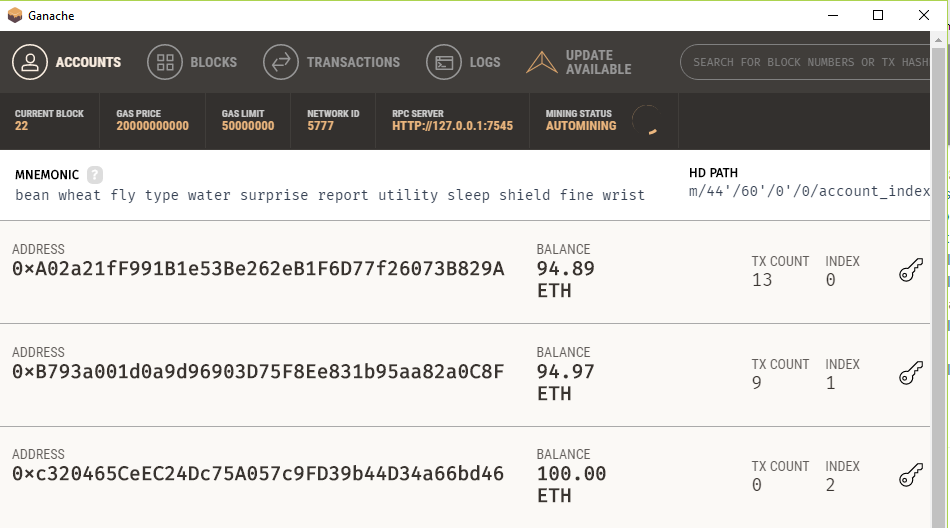
\includegraphics[width=0.5\textwidth]{ganache}
  \caption{Ganache}
\end{figure}
\section{Herramientas utilizadas para el funcionamiento de la página web, funcionando con base de datos}

\subsection{\textit{Visual Studio Code}}

Visual Studio Code\cite{VisualStudio} es un editor de texto con el cual hemos realizado gran parte de nuestro proyecto, tanto para el HTML como para la realización de los contratos una vez pasados por la plataforma Remix así como para realizar los procesos correspondientes para coger formato de nuestro contrato con JSON.

Nos decantamos por usar Visual Stuido\cite{VS-code} code ya que la edición de código no está limitada para los programas C\# o Visual Basic, sino que acepta mas programas como php, html, solidity \ldots que son los principales percusores de nuestro trabajo final. 

Otra parte positiva de este editor es la función ``IntelliSense'', la cual permite al usuario de este programa poder ahorrar tiempo al escribir instrucciones, ya que tiene una función de auto-completar con el propio editor, esto logra hacer que el trabajo sea mas productivo, acortar la escritura y no cometer errores por la sintaxis.

\subsection{\textit{XAMPP}}

La siguiente herramienta de la que hablaremos será de la creación de la base de datos, en este caso hemos querido usar XAMPP\cite{xampp}(X\footnote{X: hace referencia a que sirve para cualquiera de los diferentes sistemas operativos} Apache, MySQL, PHP, Perl.)

En el apartado 5, ``Aspectos relevantes del desarrollo del proyecto'' y en los anexos hablaremos mas específicamente sobre este programa. Explicaremos cómo realizar la instalación y el uso que le damos en nuestra aplicación. Por el momento daremos una breve introducción de por qué hemos seleccionado esta en vez de otro programa similar.

Una vez lo tengamos instalado, podremos realizar crear, editar, consultar y gestionar bases de datos en MySQL de una manera eficaz y limpia.

Al usar este programa, hemos retomado cómo poder administrar las bases de datos y su acceso a una base de datos desde PHP, así como realizar diferentes SELECT y sacar el resultado por página web.

\section{Control de versiones y documentación}

En el siguiente apartado veremos las herramientas que utilizamos para el control de las versiones y la herramienta empleada para el desarrollar del documento de este proyecto.

\subsection{\textit{Látex}}

\textit{LaTeX}\cite{latex} es un sistema de preparación de documentos. Con este programa podemos cartas, tesis, presentaciones y cualquier tipo de documento que quisieras imprimir en papel o mostrar en pantalla. 

La principal opción por la que usamos \textit{LaTex} es porque tiene una mejor calidad de tipografía en comparación con los editores convencionales.

Para el proyecto usamos \textit{TexMaker} en la versión para \textit{Windows}.

\subsection{\textit{GitLab}}

\textit{Gitlab}\cite{gitlab} es un servicio web de control de versiones y desarrollo de software colaborativo basado en \textit{Git}.

Utilizamos este programa para mostrar el proyecto finalizado. El repositorio se tendrá acceso en el siguiente repositorio. \cite{repositorio}

%\begin{figure}[h]
%    \centering
%    \includegraphics[width=0.5\textwidth]{gitLab}
%	\caption{{Logotipo del programa \textit{GitLab}}}
%\end{figure}
%\begin{wrapfigure}{r}{0.4\linewidth}
%    \centering
%    \includegraphics[width=0.20\textwidth]{gitLab}
%    \caption{Logotipo del programa \textit{GitLab}}
%\end{wrapfigure}


\capitulo{5}{Aspectos relevantes del desarrollo del proyecto}

En este apartado se van a mostrar los aspectos más importantes del
proyecto y los procesos que hemos seguido para el correcto funcionamiento de nuestra pagina con la debida conexión con la red Ethereum. Hablaremos de las herramientas utilizadas, pero la instalación de la mismas y la finalización de la página lo comentaremos en el apartado de los anexos.

El trabajo comenzó con la visita de la compañía HP a la universidad a exponer y realizar una charla sobre los TFG que se podían realizar con ellos durante el curso, para así empezar a realizar trabajos con una empresa real para un trabajo determinado.

\section{Comienzo del proyecto}

El trabajo comienza a partir de un proyecto que propone la empresa HP(Hewlett Packard) sobre aplicación de tecnología Blockchain a una cadena de distribución de productos. 

Una vez realizamos las primeras sesiones de para conocer al tutor de la empresa de HP: Pablo Tejedor García.

En la primera sesión decidimos los tiempos para realizar las diferentes tareas y ver la complejidad de cada una de ellas, todas las reuniones han sido realizadas vía llamada remota o presencialmente en la sede de León.

\section{Primeras sesiones}

En la primera sesión me recomendó la lectura del libro \textit{[Scrum y xp desde las trincheras]} el cual hemos comentando anteriormente, y la realización de programas básicos de prueba para la realización de la página en Visual Studio ya que le dije que habíamos usado esta herramienta durante la carrera y según algunos artículos era posible la conexión con la tecnología Blockchain, mediante la red web3 y la aplicación de la cual hablaremos mas adelante Metamask.


\section{Primer contacto con \textit{Ethereum}}

Una vez acabado y resumido el libro y realizados los primeros programas con Visual Studio, dimos el paso a la realización de nuestros primeros \textit{smart contract} 

En primer lugar, se decidió realizar un tutorial para tener unas tomas básicas en el ámbito de los \textit{smart contract}, ya que era la primera vez que utilizaríamos este tipo de lenguaje.

Este tutorial se realiza entero mediante Internet, se trata de una serie de capítulos los cuales te enseñan desde cero la creación de un contrato Solidity.

Hablaremos de ello en el apartado de trabajos relacionados en el punto siguiente.

\begin{figure}{l}
  \centering
  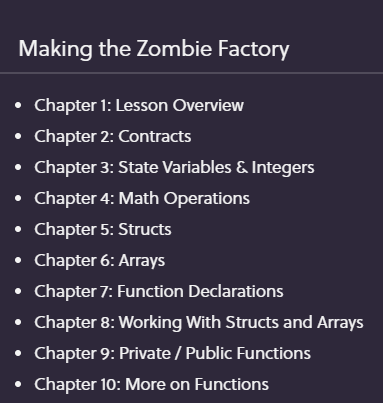
\includegraphics[width=0.5\textwidth]{zombie}
  \caption{Funciones: CryptoZombies}
\end{figure}  

Una vez concluido este proceso de iniciación en el mundo de Solidity, el siguiente paso era realizar pequeños contratos con cambio de dinero entre cuentas Ethereum, pero para empezar todas estas operaciones las realizamos mediante la opción localHost, esto lo conseguimos mediante dos formas.

\section{Realización de contratos en modo \textit{LocalHost}}

Para la realización de esto se empezó a usar una página de la cual no nos separemos a lo largo de nuestro proyecto, Remix.

Gracias a esté sitio web los smart contract que creemos se podrán probar directamente mediante la compilación.

Podremos seleccionar la versión con la que estamos trabajando y una vez compilado y sin errores, iremos a la pantalla de \textit{DEPLOY \& RUN TRANSACTIONS} una vez en esta página tendremos varias opciones 

En la opción \textit{Enviroment}, podremos elegir como se realizaran nuestros contratos:
\begin{itemize}
	\item JavaScript VM: esto nos crea 5 cuentas con una cantidad de 100 Ether en cada una, esto será una opción local para pequeñas pruebas, cuando cerreremos o ejecutemos otro programa la cuenta volverá a reiniciarse.
	\item Injected Web3: esta opción nos conectará directamente con Metamask, una vez que demos a \textit{deploy}, desplegar.
	\item Web3 Provider: en esta opción nos conectará con el servidor local de Ganache y nos dará acceso a las 10 cuentas que hay disponibles.
\end{itemize}
Con todas estas opciones nos creará un primer contrato, sin ningún valor mas que el gas de transacción.

Gracias al desplegable Account podremos seleccionar la cuenta en la que estemos, siempre y cuando no estemos en Injected Web3, ya que con esta opción siempre manejaremos la red desde Metamask.

Otro apartado es Gas limit se podrá indicar cuanto queremos y en caso de no poner un valor que sea inferior, nos mostrara error en este apartado. 

El ultimo parámetro que se puede modificar sera el valor que queremos indicar (Wei, Gwei o Ether), en caso de que nuestro contrato tenga una cantidad de divisa a enviar y no pongamos el valor, nos mostrará error de cantidad invalida.  

\begin{figure}[h]
  \centering
  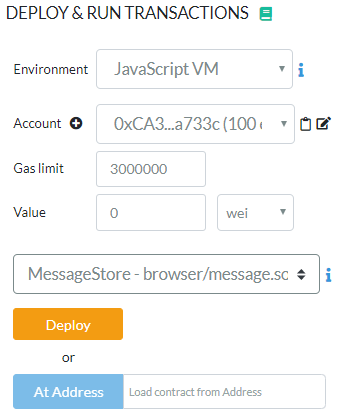
\includegraphics{remix-contract}
  \caption{Ejecutar contrato desde Remix}
\end{figure}  

\section{Creación de contratos desde Visual Studio}

Una vez fue entendida la herramienta con Remix, el siguiente paso fue la creación de una DApps, con las herramientas Visual Stuido, Tuffle, node.js y Ganache.

Primeramente tendríamos que instalar Node.js (\url{https://nodejs.org/en/}), una vez que fuera instalada instalaremos Truffle, y a continuación crearemos o ejecutaremos una carpeta  la cual contendrá los siguientes archivos:
\begin{itemize}
	\item contracts/: contiene los archivos Solidity que tendrán los contratos inteligentes.
	\item migratios/: sistema utilizado por Truffle para manejar las implementaciones de los smart contract. 
	\item test/: aquí realizaremos las pruebas Solidity y JavaScript para los smart contract
	\item truffle-config.js: archivo de configuración de Truffle.
\end{itemize}

Una vez tengamos la carpeta creada, escribiremos los smart contract, indicando la versión que deseemos usar de Solidity, cuando este finalizado nos encargaremos de compilar (truffle compile), y a continuación los migraremos\footnote{Migración: \textit{script} de implementación creado para alterar el estado de los contratos de su aplicación.} a nuestra cadena de bloques.

Anteriormente hablábamos de la herramienta Metamask, ahora para la conexión de desde Visual Studio a nuestro contrato, será necesario la instalación, la podremos descargar desde \url{https://metamask.io/}, es una extensión disponible para Chrome, Firefox, Opera, Brave, iOS y Android. También necesitaremos la aplicación Ganache, \url{https://www.trufflesuite.com/ganache}, este programa nos surtirá en modo local de diez cuentas, para poder trabajar con ellas, pero una vez que cerremos todo lo realizado de las transacciones se perderá.

El proceso de instalación de las herramientas anteriormente mencionadas lo comentaremos en el apartado de anexos.

Una vez tengamos Metamask tendremos que se crear o seleccionar la cuenta localhost:7545 será la encargada de conectar con Ganache, importando previamente las cuentas (con el código privado de la clave). 

Una vez tengamos todos creado, desde la terminal de Visual Studio (ctrl+ñ) tendremos que ejecutar npm run dev esto hará que el servidor se inicie y abra una pestaña en el navegador con el contenido de la dapp.

\begin{figure}[h]
  \centering
  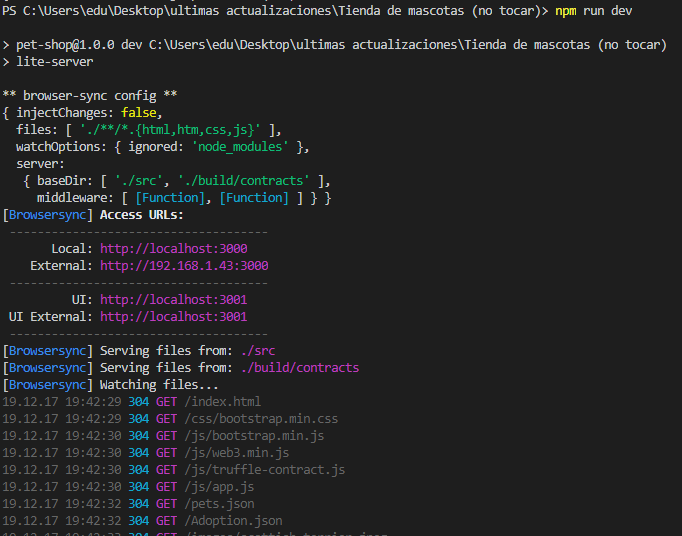
\includegraphics[width=1.00\textwidth]{npmrundev}
  \caption{Muestra de la ejecucción desde Visual Studio}
\end{figure}  

\section{Programas creados antes del programa final}

Antes de la creación final hemos realizado dos programas, ambos con conexión perfecta en ganache desde metamask, pero al intentar modificar las redes y tener que usar una red principal o privada, surgieron los mayores problemas, bien por problemas de divisa en Ether en las cuentas (debido a su dificultad de conseguir esta moneda en las redes, recordamos que en las redes locales que manejábamos anteriormente las divisas nunca se acaban ya que si reiniciamos la cuenta el dinero volvería al estado inicial de 100 Ether).

Los archivos que hemos creado son un servicio de compra de autobuses y una tienda de mascotas

\section{Empezando con redes privadas}

Al finalizar los contratos mediante la red con Ganache y comprobar que se realizaban correctamente el siguiente paso que nos propusimos fue la conexión de los smart contract con una red privada como son Ropsten, Rinkeby, Kovan.

Lo primero que hay que hacer es ingresar Ether en la cuenta, investigando por Internet descubrimos que había una página la cual permitía recaudar dinero pero solamente para la red Rinkeby.

El proceso para conseguir Ether consta de las siguientes partes:
\begin{enumerate}[1]
	\item Iremos a la página \url{https://plus.google.com/}, también se podrá realizar mediante la red de Twitter o Facebook y ahí tendremos que publicar el número de cuenta donde deseemos recibir el Ether.
	\item Una vez publicado copiaremos la url de nuestro post.
	\item Por ultimo en la pagina \url{https://www.rinkeby.io/#faucet} pegaremos la url y seleccionaremos el Ether que deseemos recibir, dependiendo la cantidad que escojamos no podremos realizar una nueva petición hasta que pasen los días  establecidos.
	\item Cuando se complete el proceso, podremos comprobar la cuenta y comprobar que el Ether aumento la cantidad seleccionada previamente.
\end{enumerate}

Ahora que ya tenemos dinero en nuestra red, podremos empezar a realizar smart contract desde Visual Stuido y conectar con las redes privadas mediante la aplicación que hace de intermediaria llamada Metamask. 
	 
\section{Problemas de conexión Web3}

En este punto en el cual ya disponíamos de dinero en nuestra red, intentamos la realización de poder ejecutar desde Visual Stuido a la red Ethereum, pero ya no en modo local como usábamos Ganache, si no realizarlo con Web3 y que realizara la conexión o con una red pública o privada.

Esto nos llevo mas de un quebradero de cabeza, ya que la conexión nos daba errores, por problemas de versiones de nuestro solidity y por asíncronos.

Nos planteamos el realizar una base de datos, la cual recogiera todos los datos y estos poder mostrarlos posteriormente, esto sin poder enseñarlos en la página de Etherscan.

Pero investigando y probando resulto que con la red privada Ropsten si que era posible realizar los contratos.

\section{Creación de la página}

Después de haber comprobado que nos permitía realizar los contratos de forma correcta y en la red privada, llego el momento de realizar la página web.

La cual hemos realizado con el programa XAMPP, es sistema de gestión de base de datos en MySQL y con Visual Stuido.

La pagina web hemos creado estas pantallas:
\begin{enumerate}[a]
	\item Inicio de sesión
	\item Nueva cuenta
	\item He olvidado la contraseña
	\item Mostrar opciones
	\item Añadir producto
	\item Consultar último producto
	\item Consultar productos existente
	\item Administrador de la cuenta
	\item Modificar datos del propio usuario
\end{enumerate}

Hablaremos más detenidamente del \textit{font-end} y \textit{back-end}, así como de la instalación de XAMPP en el apartado de los anexos.

\capitulo{6}{Trabajos relacionados}

En este apartado tendremos la oportunidad de hablar acerca de trabajos similares al que hemos realizado en este proyecto. 

Ya que no hay ninguno que se relacione con trabajos de la universidad de Burgos, hablaremos sobre los encontrados en Internet y los que se realizan en la empresa HP.

Al comenzar el trabajo final, el tutor académico me pregunto sobre mi conocimiento de Blockchain y la programación con Solidity, al ser principiante con esta tecnología me insto a seguir estos cursos para empezar a familiarizarme con este tipo de programación:

\paragraph{\textit{CryptoZombies}}\cite{crypto}: es una página, en la cual, tienes que seguir una serie de capítulos en la cual te enseñan la programación para la creación de contratos inteligentes en Solidity. 

Enseñan los conceptos básicos y los tipos de variables que hay, a demás de como implementar funciones y poder ejecutarlas.


\paragraph{\textit{Pet-shop}}\cite{shop}: tenemos un tutorial, el cual, nos explicará como poder crear una Dapp, y sera un sistema para poder adoptar mascotas. Nos enseña la utilización de:

\begin{itemize}
	\item Configurar el desarrollo en el que trabajaremos.
	\item Configurar un proyecto con Truffle.
	\item Escribir nuestro propio \textit{smart contract}.
	\item Compilación del \textit{smart contract}.
	\item Migrar y ejecutar el \textit{smart contract}.
	\item Crear la interfaz de usuario.
	\item Interactuar con metamask para dar los pasos para la compra de la mascota.
\end{itemize}

\paragraph{\textit{Crypto Kitties}}: es una de una de las grandes aplicaciones con mas fama en el mundo de las \textit{DApps}.

Con esta aplicación tendremos una familia de gatos ``digitales''\cite{gatos}, y el gato que se forme podrá valer una cierta cantidad dependiendo sus cualidades. 

Cabe destacar que cada gato en esta página es un \textit{token} indivisible de Ethereum, así que cualquier compra, venta o transacción que se pueda realizar conllevara un  gasto de minería.

Para poder interacutar con esta aplicación tendremos que tener instalado el plugin de Metamask y una cuenta con Ether suficiente para poder realizar las operaciones deseadas.

\paragraph{\textit{Brave}}\cite{brave}: es un navegador web de código abierto el cual esta basado en \textit{Chromium}\footnote{\textit{Chromium}:\cite{chromium} es un navegador web gratuito y de código abierto desarrollado por Google.}.

Este navegador tiene la capacidad de bloquear los anuncios(incluso lleva una cuenta de cuantos anuncios bloqueo) y una gran cantidad de rastreadores en linea, y asegura proteger la privacidad de los usuarios, reduciendo los datos con los anunciantes.

Según anuncian en la sus redes \textit{Brave} es mas rápido que sus competidores, Chrome y Safari, en ordenadores es dos veces mas rápido y en dispositivos móviles puede llegar a ser hasta ocho veces mas rápido.

Tiene también versión para móvil en las versiones de Android y iOS.

\paragraph{\textit{Aragon}}: es un proyecto que pretende eliminar los intermediarios en el proceso de creación y mantenimiento de estructuras organizativas. Esto es posible a través del uso de la cadena de bloques.


\section{Empresas y organizaciones que usan \textit{blockchain}}

Hay múltiples empresas que han empezado a utilizar la tecnología \textit{blockchain} en el día a día para mejorar la gestión u ofrecer al publico un servicio de más calidad.

A continuación, expondremos algunos ejemplos de estas empresas\cite{empresas}, las cuales las podremos dividir en diferentes sectores como: 
\subsection{Comercio}
\begin{itemize}
	\item \underline{\textit{Walmart}}: es una multinacional que quiere aprovechar el registro digital para mejorar las gestiones y los seguimientos de datos para usar en el día a día. 
\end{itemize}
\subsection{Envío de paquetería}
\begin{itemize}
	\item \underline{\textit{FedEx}}: una empresa de envíos que permite mejorar el proceso de resolución de disputas con los clientes. Quiere usarlo para identificar el tipo de datos, almacenarlo en una \textit{blockchain} y también para almacenar registros en futuros envíos o problemas.
\end{itemize}

\subsection{Protección de datos}
\begin{itemize}
	\item \underline{\textit{Facebook}}: explora el uso de \textit{blockchain} para mejorar la seguridad de los datos y poder ofrecer mayor seguridad a los usuarios.
	\item \underline{\textit{Google}}: realiza la misma operación que Facebook para poder proporcionar seguridad a todos sus usuarios.
\end{itemize}
\subsection{Transporte}
\begin{itemize}
	\item \underline{\textit{British Airways}}: lo realiza para administrar la información sobre los vuelos mas importantes en el aeropuerto de Londres y Miami. Con ello verifican la identidad de las personas que viajan en el vuelo, mediante la base de datos que se encuentra en \textit{blockchain}. 
	\item \underline{\textit{Toyota}}: para mejorar la conducción autónoma. 
\end{itemize}
\subsection{Bancos}
\begin{itemize}
	\item \underline{\textit{MasterCard}}: la compañía de \textbf{EE. UU.} lo utiliza para realizar los pagos de forma instantánea.
    \item \underline{\textit{BBVA}}:  también quiere conseguir la rápida circulación de la moneda mediante la transferencia. 
	\item \underline{\textit{Banco Santander}}: tiene una aplicación que ejecuta pagos internacionales, mediante los dispositivos móviles (\textit{smartphones}). La transferencia puede ser efectiva en torno a los 40 segundos. 
\end{itemize}







\capitulo{7}{Conclusiones y Líneas de trabajo futuras}

\section{Conclusiones}

Tras haber finalizado con la realización del proyecto, podemos decir que hemos cumplido la mayoría de los objetivos y los requisitos que se propusieron al iniciar el mismo.

El objetivo principal, era la creación de contratos inteligentes en la red Ethereum o las redes privadas que ofrece esta misma, mediante una página web, en un principio hemos trabajado todo mediante la red Localhost, con la posibilidad de en un futuro crear un dominio y que fuera de ámbito general.

Gracias a la investigación y realización de este proyecto, he aprendido a usar nuevos lenguajes de programación (Solidity, React, Ethereum) y a coger experiencia en otros que ya había visto en la carrera pero con apenas experiencia en ellos (HTML, CSS, PHP). 

En otro caso, gracias a la colaboración de HP en este proyecto de investigación, he aprendido el funcionamiento de una empresa. También nos hemos encontrado con limitaciones en el desarrollo del proyecto, ya que al no estar tan desarrollada la tecnología sobre blockchain, la información no era tan abundante en las redes como en otros lenguajes de programación.

Como apunte final, cabe destacar que los problemas o errores encontrados durante la realización del proyecto, me han ayudado a investigar e intentar buscar soluciones de forma más o menos efectiva dependiendo del error. Este proyecto ha sido un proceso de auto aprendizaje contando con la ayuda de Pablo Tejedor (tutor de HP) y de Ángel Arroyo (Tutor académico).  

\section{Líneas de trabajo futuras}

Posibilidades de expansión

\begin{itemize}
	\item Ampliación del catalogo CNAE para dar mayor especificación al producto.
	\item Ampliación de la aplicación para no usar solo la red ethereum sino también otras blockchain públicas o privadas.
	\item Creación de un sistema de usuarios ampliado (diferentes tipos de empresa según su sector de actividad).
	\item Mejoras visuales de la aplicación.
	\begin{enumerate}[a)]
		\item Tracking del producto (incorporación de servicio de mapas tipo Google Maps a la app). usar marcado GPS.
		\item Añadir fotografía del producto añadido.
		\item Anexar documentación oficial sobre el producto y introducirlo en la blockchain.
	\end{enumerate}
	\item Publicar la página en servicio en linea, así la pagina estará siempre disponible para su uso.
\end{itemize}





\bibliographystyle{plain}
\bibliography{bibliografia}

\end{document}